\documentclass[12pt,a4paper,openright]{report}
\usepackage[italian]{babel}
\usepackage{newlfont}
\usepackage{color}
\textwidth=450pt\oddsidemargin=0pt

\usepackage{setspace}
\usepackage[utf8]{inputenc}
\usepackage{hyperref}
\usepackage{amsmath, amsthm, amssymb, mathtools}
\usepackage{enumitem}
\usepackage{physics}
\usepackage{empheq, bm}
\usepackage{graphicx}
\usepackage{float}
\usepackage{verbatim}
\usepackage{upgreek}
\usepackage[dvipsnames]{xcolor}
\newcommand{\virgolette}[1]{``#1''}
\usepackage{soul}
\newcommand{\figref}[1]{figura \ref{#1}}
\newcommand{\tabref}[1]{tabella \ref{#1}}
\renewcommand{\eqref}[1]{equazione \ref{#1}}
\numberwithin{equation}{section}
\numberwithin{figure}{section}
\numberwithin{table}{section}
\DeclareMathOperator{\sen}{sen}
\DeclareMathOperator{\senc}{senc}
\renewcommand{\thefootnote}{\fnsymbol{footnote}}
\renewcommand{\Vec}{\bm}
\hypersetup
   {
   %bookmarks=true,         % show bookmarks bar?
    unicode=false,          % non-Latin characters in Acrobat’s bookmarks
    pdftoolbar=true,        % show Acrobat’s toolbar?
    pdfmenubar=true,        % show Acrobat’s menu?
    pdffitwindow=false,     % window fit to page when opened
    pdfstartview={FitH},    % fits the width of the page to the window
    pdftitle={Tesi triennale},   % title
    pdfauthor={Simone Chiarella},     % author
    pdfsubject={Segmentazione automatica di immagini TC},   % subject of the document
    pdfcreator={Simone Chiarella},   % creator of the document
   %pdfproducer={Producer}, % producer of the document
   %pdfkeywords={keyword1, key2, key3}, % list of keywords
    pdfnewwindow=false,      % links in new PDF window
    colorlinks=true,       % false: boxed links; true: colored links
    linkcolor=blue,          % color of internal links (change box color with linkbordercolor)
    citecolor=red,        % color of links to bibliography
    filecolor=magenta,      % color of file links
    urlcolor=cyan,           % color of external links
   %urlbordercolor={1 1 1}  % color of border around links
   }

\newenvironment{sistema}% 
{\left\lbrace\begin{array}{@{}l@{}}}% 
{\end{array}\right.}

%\usepackage[backend=biber, natbib=true, style=numeric-comp, sorting=none, doi=false, url=true, isbn=true, hyperref = true]{biblatex}

\usepackage[backend=biber, natbib=true, style=phys, citestyle=numeric, biblabel=brackets, sorting=none, doi=false, url=false, block=space, backref=true, backrefstyle=two, abbreviate=true, isbn=true, hyperref = true]{biblatex}
\usepackage[autostyle, italian=guillemets]{csquotes}
\addbibresource{biblio.bib}

\begin{document}

\begin{titlepage}
%
%
% UNA VOLTA FATTE LE DOVUTE MODIFICHE SOSTITUIRE "RED" CON "BLACK" NEI COMANDI \textcolor
%
%
\begin{center}
{{\Large{\textsc{Alma Mater Studiorum $\cdot$ Universit\`a di Bologna}}}} 
\rule[0.1cm]{15.8cm}{0.1mm}
\rule[0.5cm]{15.8cm}{0.6mm}
\\\vspace{3mm}

{\small{\bf Scuola di Scienze \\ 
Dipartimento di Fisica e Astronomia\\
Corso di Laurea in Fisica}}

\end{center}

\vspace{20mm}

\begin{center}\textcolor{black}{
%
% INSERIRE IL TITOLO DELLA TESI
%
\begin{spacing}{2}
{\LARGE{\bf SEGMENTAZIONE AUTOMATICA DI IMMAGINI TC PER LO STUDIO DELLA COMPOSIZIONE CORPOREA}}\\
\end{spacing}
}\end{center}

\vspace{30mm} \par \noindent

\begin{minipage}[t]{0.47\textwidth}
%
% INSERIRE IL NOME DEL RELATORE CON IL RELATIVO TITOLO DI DOTTORE O PROFESSORE
%
{\large{\bf Relatore: \vspace{2mm}\\\textcolor{black}{
Prof.ssa Claudia Testa}\\\\
%
% INSERIRE IL NOME DEL CORRELATORE CON IL RELATIVO TITOLO DI DOTTORE O PROFESSORE
%
% SE NON AVETE UN CORRELATORE CANCELLATE LE PROSSIME 3 RIGHE
%
\textcolor{black}{
\bf Correlatore:
\vspace{2mm}\\
Dott. David Bianchini\\\\}}}
\end{minipage}
%
\hfill
%
\begin{minipage}[t]{0.47\textwidth}\raggedleft \textcolor{black}{
{\large{\bf Presentata da:
\vspace{2mm}\\
%
% INSERIRE IL NOME DEL CANDIDATO
%
Simone Chiarella}}}
\end{minipage}

\vspace{30mm}

\begin{center}
%
% INSERIRE L'ANNO ACCADEMICO
%
Anno Accademico \textcolor{black}{ 2020/2021}
\end{center}

\end{titlepage}

\shipout\hbox{}
\begin{abstract}
Segmentare un’immagine significa riconoscere al suo interno elementi con caratteristiche comuni e raggrupparli, distinguendoli dagli elementi che posseggono caratteristiche diverse; si parla di segmentazione automatica quando questo processo è eseguito completamente da un software senza l’intervento umano. Segmentare le immagini TC, molto diffuse in ambito diagnostico, permette di estrarre una grande quantità di dati dall’alto valore prognostico e predittivo della composizione corporea del paziente. Tuttavia, a causa della scarsa diffusione di software per la segmentazione automatica, tutti questi dati non vengono utilizzati.

Il presente lavoro di tesi si propone di riportare lo stato dell’arte sulla segmentazione, sia manuale sia automatica, dei tessuti corporei in immagini TC. Vengono spiegati i vantaggi dell’utilizzo di grandezze \textit{CT-derived} rispetto a molti dei protocolli odierni e vengono esposti gli attuali livelli di accuratezza delle segmentazioni effettuate con metodi automatici. Inoltre, ci si sofferma, cercando di quantificarli, sugli effetti del mezzo di contrasto sulle grandezze \textit{CT-derived}, poiché questi possono generare errori nella segmentazione automatica dei tessuti. Infine, viene esposto l’approccio 3D alla segmentazione in contrapposizione al metodo \textit{single slice}, con il primo caratterizzato da un’accuratezza maggiore del secondo.
\end{abstract}
\shipout\hbox{}

\tableofcontents
\clearpage
\null
\newpage

\chapter*{Introduzione}
\addcontentsline{toc}{chapter}{Introduzione}
La tomografia computerizzata (TC) è una tecnica diagnostica fondata, come la radiografia, sull'assorbimento di raggi X, ma rispetto alla tradizionale radiografia proiettiva, la TC ha il vantaggio di generare immagini volumetriche. La TC riesce a mettere in evidenza dettagli che altrimenti non sarebbe possibile notare da una semplice serie di immagini radiografiche proiettive. Un'altra differenza fondamentale è il passaggio dal pixel al voxel, il che risolve le ambiguità dovute alla sovrapposizione di diversi oggetti lungo una direzione, non distinguibili in radiografia. Il principio di ricostruzione dell'immagine nella TC è piuttosto semplice: si tratta di acquisire immagini radiografiche da direzioni diverse e metterle insieme per individuare il punto nello spazio in cui è collocato l'oggetto che ha generato l'attenuazione. Ciò è possibile grazie alla rotazione completa del \textit{gantry}, cioè il dispositivo che contiene il tubo a raggi X, in una traiettoria che risulta essere ad elica attorno al paziente, posto su un lettino motorizzato.

La TC è una tecnica diagnostica incredibilmente versatile, infatti può essere utilizzata per diagnosticare diverse patologie o effettuare valutazioni cliniche, come lo studio della densità ossea, correlata all'osteoporosi, la stima del grado di obesità e di sarcopenia del paziente. Come altre tecniche radiografiche anche in TC è possibile utilizzare mezzi di contrasto per poter evidenziare \textit{uptake} di strutture di interesse. Possedere informazioni su queste condizioni cliniche è importante per la valutazione dei fattori di rischio, per la formulazione di strategie per ridurlo e per il loro valore prognostico in persone già affette da altre malattie.

Spesso le informazioni delle indagini TC sono acquisite per scopi non diagnostici, come nel caso della PET/TC o della TC di centratura radioterapica. Queste informazioni sono preziose per studiare i volumi dei tessuti corporei evitando di esporre il paziente a esami specifici, senza costi aggiuntivi per la struttura ospedaliera né ulteriore assorbimento di radiazioni al paziente stesso. Quasi mai queste informazioni vengono utilizzate, sebbene siano preziose perché possono essere usate per classificare i tessuti del paziente estratti dalle immagini mediante un procedimento noto come segmentazione.

Segmentare un’immagine significa riconoscere al suo interno elementi con caratteristiche in comune, distinguere questi elementi da altri con caratteristiche diverse e raggruppare tutti gli elementi simili in regioni, delineando dei bordi tra di esse. In un’immagine digitale, la segmentazione consiste nel classificare e quantificare in qualche modo le proprietà di ciascun pixel, come l’intensità, il colore e la \textit{texture}. Sebbene possa sembrare un’operazione semplice, effettuare manualmente un lavoro di segmentazione su una serie di immagini TC è un processo ripetitivo, operatore-dipendente e che richiede parecchio tempo. Da qui nasce l’esigenza di un metodo automatizzato, fondato sull'utilizzo di reti neurali, per segmentare i diversi tessuti del corpo umano.

Lo scopo di questa tesi è quello di riportare lo stato dell'arte sulla segmentazione, sia manuale sia automatica, dei tessuti corporei in immagini TC, spiegando tutti i vantaggi dell'utilizzo di grandezze \textit{CT-derived} rispetto a molti dei protocolli odierni ed esponendo gli odierni livelli di accuratezza delle segmentazioni effettuate con metodi automatici. Inoltre, ci si sofferma, cercando di quantificarli, sugli effetti del mezzo di contrasto sulle grandezze \textit{CT-derived}, poiché questi possono generare errori nella segmentazione automatica dei tessuti. Infine, viene esposto l'approccio 3D alla segmentazione in contrapposizione al metodo \textit{single slice}, dove il primo è caratterizzato da un'accuratezza maggiore del secondo.

L'esposizione degli argomenti è articolata come segue.
\begin{description}
\item[Il primo capitolo] contiene le informazioni preliminari necessarie per comprendere a pieno il contenuto dei capitoli successivi, quali la tecnologia della tomografia computerizzata, le basi teoriche della segmentazione, un'introduzione alle reti neurali, in particolare quelle a convoluzione, e alcuni metodi statistici.
\item[Il secondo capitolo] espone gli obiettivi e l'utilità dello studio della composizione corporea, illustrando anche i vantaggi derivanti dall'utilizzo di immagini TC e di grandezze \textit{CT-derived} rispetto ai protocolli odierni di stima della \textit{body composition}; contemporaneamente viene sottolineata la necessità di metodi di segmentazione automatica per permettere il pieno utilizzo delle informazioni contenute all'interno delle TC.
\item[Il terzo capitolo,] infine, contiene lo stato dell'arte sulla segmentazione automatica dei tessuti corporei, una panoramica sugli effetti del mezzo di contrasto sulle grandezze \textit{CT-derived} e un accenno all'approccio 3D per la stima della \textit{body composition}.
\end{description}



\chapter{Materiali e metodi}
Il presente capitolo ha lo scopo di fornire tutto un insieme di informazioni preliminari utili a comprendere meglio i capitoli successivi, i quali rappresentano il vero corpo di questo lavoro di tesi. Innanzitutto viene presentata un'introduzione all'acquisizione di immagini radiografiche e alla tomografia computerizzata, mettendo in luce le differenze tra due tecniche fondate entrambe sull'attenuazione di raggi X da parte dei tessuti del corpo, ma nonostante ciò profondamente diverse. Successivamente vengono riportate in breve le basi teoriche della segmentazione e delle reti neurali impiegate nella segmentazione automatica. Infine si passa all'esposizione dei principali metodi statistici impiegati negli studi utilizzati per questa tesi.

\section{Formazione di un'immagine a raggi X}
La formazione di un'immagine a raggi X è la conseguenza dell'attenuazione di un fascio di raggi X a carico dell'oggetto investito dal fascio stesso. Come illustrato nella \figref{fig:apparatox}, sia prima sia dopo l'oggetto da indagare sono posti dei collimatori, in modo tale che i fotoni che arrivano sulla lastra siano sono quelli perpendicolari alla lastra stessa, dove si formerà l'immagine finale. L'attenuazione del fascio è maggiore per i tessuti duri e minore per i tessuti molli, mentre è quasi nulla per l'aria, come mostrato nella \figref{fig:radiografia}. L'attenuazione del fascio segue la legge di Lambert-Beer:
\begin{equation}\label{lambert}
    I(x) = I_0\,\mathrm{e}^{-\mu_\mathrm{l}x}\,,
\end{equation}
dove $I_0$ è l'intensità iniziale del fascio, \textit{x} è la coordinata spaziale che quantifica la distanza percorsa da un fotone all'interno di un certo materiale, e $\mu_\mathrm{l}$ è il coefficiente di attenuazione lineare del materiale per un'energia fissata del fotone. Nel caso di un fascio monocromatico emesso con intensità $I_0$ ed energia \textit{E}, che attraversa lo spessore \textit{x} di un corpo, si definisce la trasmittanza del fascio stesso come:
\begin{equation}
    T = \frac{I(x)}{I_0} = \mathrm{e}^{-\int_0^x \mu_\mathrm{l}(E,x')\,\mathrm{d}x'}\,,
\end{equation}
in cui è importante sottolineare che il coefficiente di attenuazione lineare $\mu_\mathrm{l}$ è funzione non solo dell'energia ma anche della posizione, in quanto la composizione del corpo investito dal fascio può essere varia. Inoltre, il coefficiente di attenuazione lineare dipende dal numero di massa atomica del materiale, dalla sua densità e anche dall'energia del fascio di raggi X, come si può osservare nella \figref{fig:trasmittanza}; si può dedurre che il coefficiente di attenuazione è proporzionale alla densità del materiale e inversamente proporzionale all'energia del fascio.
\begin{figure}[htp]
\centering
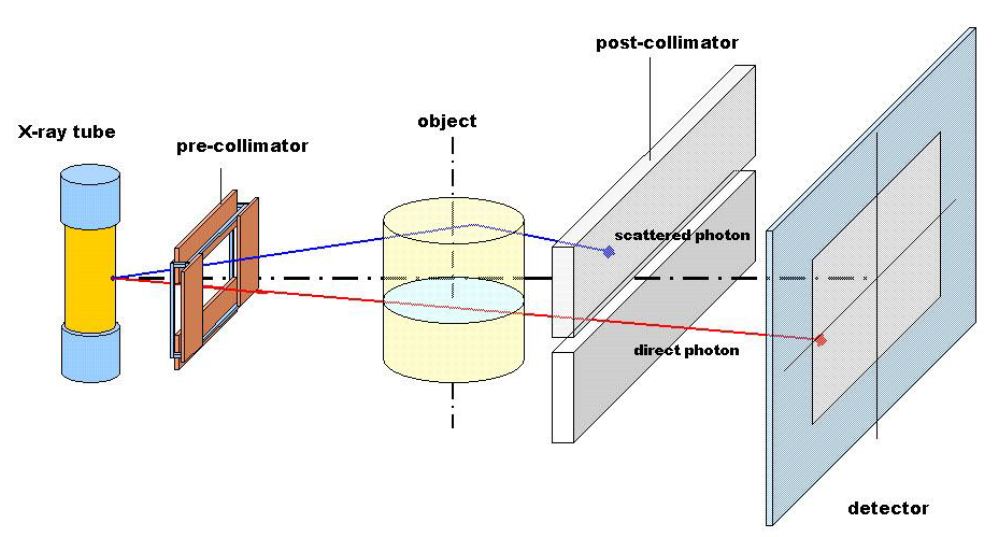
\includegraphics[scale=0.6]{Immagini/apparatox.png}
\caption{\label{fig:apparatox} \textit{Schematizzazione di un sistema per la formazione di immagini a raggi X}.}
\end{figure}
\begin{figure}[H]
\centering
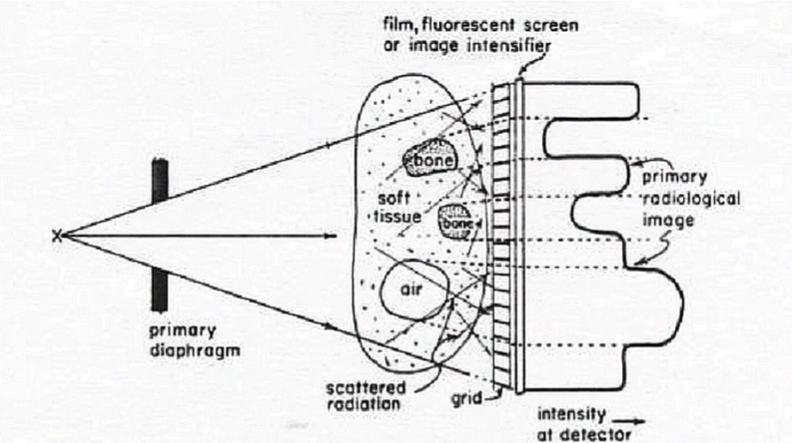
\includegraphics[scale=0.7]{Immagini/radiografia.png}
\caption{\label{fig:radiografia} \textit{Schema basilare per la formazione di immagini a raggi X}.}
\end{figure}
\begin{figure}[H]
\centering
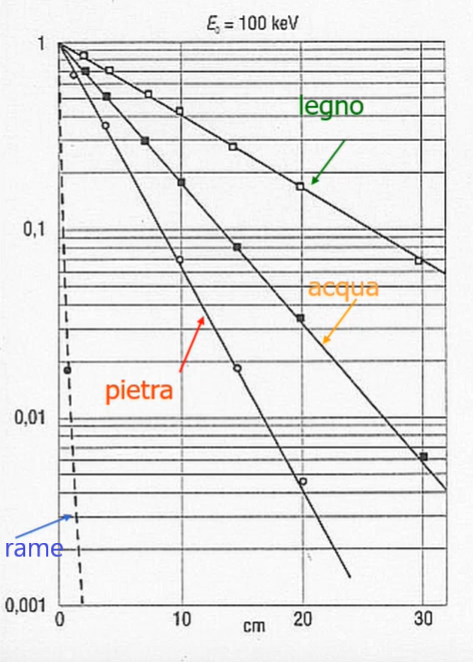
\includegraphics[scale=0.444]{Immagini/trasmittanza.png}\quad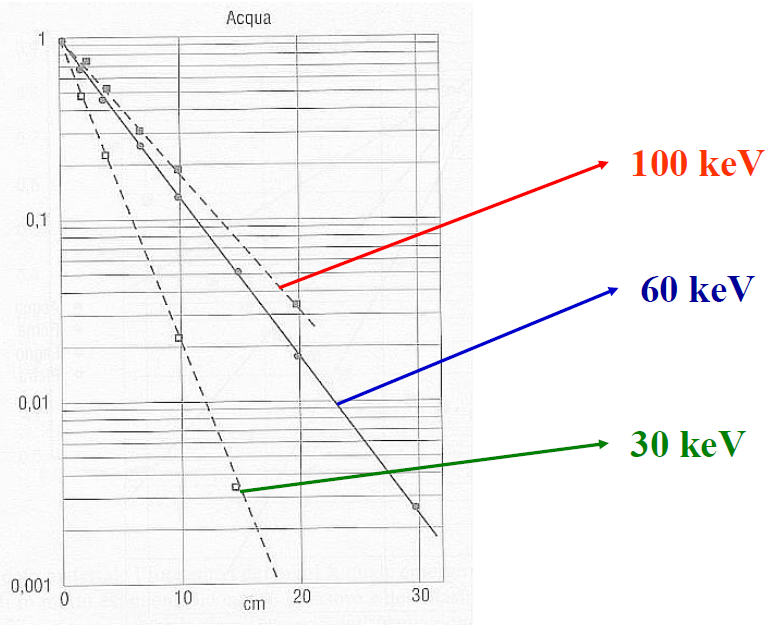
\includegraphics[scale=0.59]{Immagini/trasmittanza2.png}
\caption{\label{fig:trasmittanza} \textit{Da sinistra a destra: andamento della trasmittanza per materiali diversi a energia fissata e per energie diverse a materiale fissato}.}
\end{figure}

La dipendenza di $\mu_\mathrm{l}$ dai diversi parametri può essere espressa in funzione del coefficiente di attenuazione atomico $\mu_\mathrm{a}$ nel modo seguente:
\begin{equation}
    \mu_\mathrm{l} = \frac{\rho \mathrm{N_A}}{A} \mu_\mathrm{a}\,,
\end{equation}
dove $\rho$ rappresenta la densità del materiale, \textit{A} il numero di massa atomica degli atomi che lo compongono e $\mathrm{N_A}$ il numero di Avogadro.
Il coefficiente di attenuazione atomico ha le dimensioni di una sezione d'urto e indica la probabilità di interazione tra un fotone attraversante una superficie unitaria contenente un solo atomo e quest'ultimo. Per fotoni con energia non troppo elevata (inferiore a 1\,MeV) le interazioni con la materia possono produrre tre fenomeni distinti.
\begin{description}
    \item[Effetto fotoelettrico] È la conseguenza dell'assorbimento della radiazione da parte di un elettrone, che riceve l'energia sufficiente per sfuggire dall'atomo. L'energia della radiazione viene utilizzata in parte per rompere il legame fra l'elettrone e il nucleo, mentre la restante parte si trasforma in energia cinetica dell'elettrone.
    \item[\textit{Scattering} Compton] Si ha quando il fotone interagisce con un elettrone posto in un guscio esterno dell'atomo. Il fotone colpisce l'elettrone in un urto anelastico e viene deviato, fornendo all'elettrone l'energia necessaria per poter sfuggire dall'atomo.
    \item[\textit{Scattering} Rayleigh] In questo caso, l'urto fra il fotone e l'elettrone è elastico, di conseguenza non si ha trasferimento di energia, ma l'unico effetto che si osserva è una deviazione nella traiettoria del fotone.
\end{description}
Il coefficiente di attenuazione atomico si può scrivere come somma delle sezioni d'urto dei singoli fenomeni appena elencati, posti in ordine:
\begin{equation}
    \mu_\mathrm{a} = \tau + \sigma_\mathrm{C} + \sigma_\mathrm{R}\,.
\end{equation}
In medicina non viene utilizzata radiazione con energia superiore a 1,02\,MeV, poiché un fotone del genere, interagendo con un campo elettrostatico, avrebbe energia sufficiente per produrre una coppia elettrone-positrone. La predominanza di un fenomeno rispetto a un altro dipende sia dal numero atomico del mezzo sia dall'energia del fotone, come si può osservare nella \figref{fig:effetti}: l'effetto fotoelettrico domina a bassa energia e grande numero atomico, l'effetto Compton prevale a energie medie e tendenzialmente a numero atomico piccolo, mentre la produzione di coppie elettrone-positrone si osserva per alte energie e grande numero atomico.

\begin{figure}[htp]
\centering
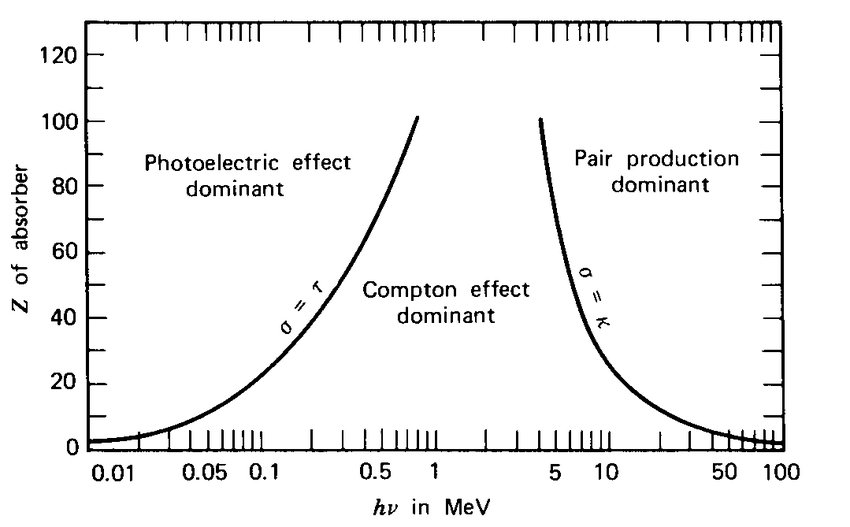
\includegraphics[scale=0.45]{Immagini/effetti.png}
\caption{\label{fig:effetti} \textit{Effetto prevalente in funzione del numero atomico del materiale e dell'energia della radiazione}.}
\end{figure}

\section{Tomografia computerizzata}
Inizialmente, con la \textbf{tomografia computerizzata} (TC) era possibile ottenere solo immagini tomografiche del piano assiale dell'organismo: per questo motivo era chiamata, e spesso lo è tuttora, tomografia assiale computerizzata (TAC), sebbene il nome corretto attualmente sia solo tomografia computerizzata.

La differenza fondamentale tra radiografia e tomografia è che la seconda è frutto di un ricalcolo e di una ridistribuzione del segnale nelle tre dimensioni, che non ha, quindi, lo scopo unico di fornire immagini radiologiche tridimensionali (tomografiche), ma riesce anche a mettere in evidenza dettagli che altrimenti non sarebbe possibile notare da una semplice serie di immagini radiografiche bidimensionali. Un'altra differenza fondamentale è il passaggio dal pixel al voxel, il che risolve le ambiguità dovute alla sovrapposizione di diversi oggetti lungo una direzione, non distinguibili in radiografia.

Il principio di ricostruzione dell'immagine nella TC è piuttosto semplice: si tratta di acquisire immagini radiografiche da direzioni diverse e metterle insieme per individuare il punto nello spazio in cui è collocato l'oggetto che ha generato l'attenuazione. Il numero di direzioni da acquisire si fonda su una regola empirica e dipende dalla risoluzione in pixel del rivelatore: il numero di direzioni di acquisizione deve essere comparabile al numero di pixel per riga del rivelatore. È inutile, perciò, acquisire un'immagine per ogni grado di angolo se si hanno, per esempio, solo 100 pixel per riga. Sebbene il coefficiente di attenuazione lineare che compare nella \eqref{lambert} dipenda sia dall'energia del fascio sia dalla densità del corpo investito, nella ricostruzione delle immagini di TC classica è spesso accettabile considerare $\mu_\mathrm{l}$ come funzione solo della densità. Ciò detto, prendendo come riferimento la \figref{fig:attenuazione}, la legge di Lambert-Beer diventa la seguente:
\begin{equation}
    I(x,y) = I_0(x,y)\,\mathrm{e}^{-\int\limits_L \mu_\mathrm{l} (x,y)\,\mathrm{d}l}\,.
\end{equation}

\begin{figure}[htp]
\centering
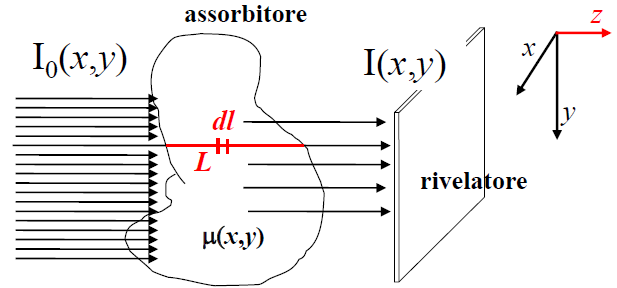
\includegraphics[scale=0.85]{Immagini/attenuazione.png}
\caption{\label{fig:attenuazione} \textit{Schematizzazione di una radiografia}.}
\end{figure}

\noindent Per ricostruire l'immagine bisogna recuperare i valori che assume il coefficiente di attenuazione lineare lungo \textit{L}; dunque, la singola radiografia è l'integrale della funzione $\mu_\mathrm{l}(x,y)$ lungo la direzione dei raggi X:
\begin{equation}\label{integralemu}
    \ln{ \left[ \frac{I(x,y)}{I_0(x,y)} \right]} = -\int\limits_L \mu_\mathrm{l} (x,y)\,\mathrm{d}l\,.
\end{equation}
A questo punto, acquisendo un'immagine con un rivelatore digitale non si ottiene un'immagine radiografica come quella delle lastre, con gli oggetti più attenuanti mostrati in bianco, bensì un'immagine dove i fotoni conteggiati vengono codificati in bianco e gli oggetti attenuanti in nero (o, per meglio dire, assenza di bianco). Da un'immagine del genere è impossibile ricavare l'integrale dell'\eqref{integralemu}, che invece si ottiene dividendo il valore d'intensità del fascio rivelato nell'immagine radiografica per il valore iniziale dell'intensità $I_0$ del fascio, che si può ottenere acquisendo un'immagine radiografica di campo vuoto; a questo rapporto si applica il logaritmo naturale. Il risultato è quello della \figref{fig:globo}, che mostra le immagini radiografiche iniziale e finale di un globo di legno. Osservando attentamente l'immagine, ad esempio nella zona in cui è presente il chiodo fra il globo e il telaio, si può vedere come l'operazione descritta dall'\eqref{integralemu} non ha il solo scopo di invertire i colori, ma ha soprattutto il compito di generare un contrasto corretto; in altre parole, se nella radiografia attenuata si è certi che due oggetti, di cui uno di gran lunga più denso dell'altro, venga riportato con il contrasto che effettivamente dovrebbe avere, nella radiografia acquisita questa certezza non c'è. L'operazione appena descritta non si può eseguire con un sistema classico di diretta incidenza dei raggi X sulla lastra.

\begin{figure}[htp]
\centering
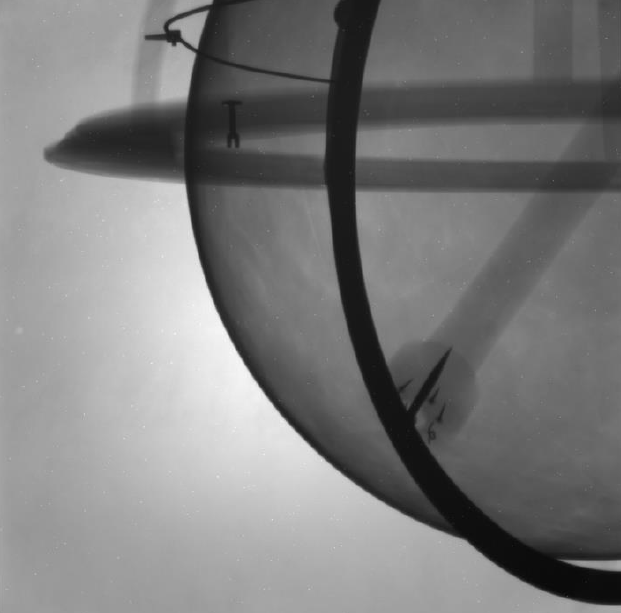
\includegraphics[scale=0.58]{Immagini/globo1.png}\quad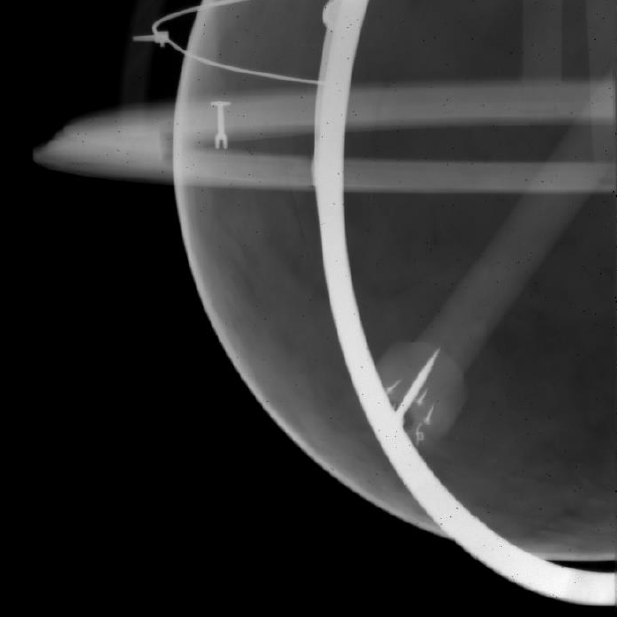
\includegraphics[scale=0.577]{Immagini/globo2.png}
\caption{\label{fig:globo} \textit{Radiografie acquisita e attenuata di un globo di legno}.}
\end{figure}

Nell'acquisizione di un'immagine radiografica è necessario anche eliminare il rumore, che appare con dei tipici puntini neri distribuiti casualmente in tutta l'immagine. Questi puntini sono dovuti a singoli raggi X che riescono a oltrepassare l'oggetto da esaminare senza interagire con esso e oltrepassano anche il rivelatore senza essere fermati, di conseguenza interagiscono direttamente con l'elettronica e vengono codificati con un'intensità estremamente elevata. Il rumore può essere eliminato con dei filtri locali, cioè metodi matematici di riduzione del rumore che prevedono la moltiplicazione dei valori d'intensità rilevata della matrice di pixel attorno a un punto per i valori di un'altra matrice detta \textit{kernel}. In pratica, si sovrappone il \textit{kernel} alla matrice dei pixel, si moltiplicano singolarmente le caselle della matrice dei pixel per le corrispondenti caselle del \textit{kernel} e si sommano tutti i valori della matrice risultante; il risultato rappresenta il valore d'intensità da assegnare al pixel al centro della matrice finale. L'operazione va ripetuta per ciascun pixel dell'immagine, attorno al quale si prenderà una certa matrice da moltiplicare sempre per lo stesso \textit{kernel}. Esistono diversi tipi di filtri, ognuno col suo \textit{kernel}, non solo per diminuire il rumore, ma anche per mettere in evidenza solo i bordi degli oggetti raffigurati nella radiografia, tralasciando l'immagine interna ai bordi qualora non sia utile, e anche per mettere a fuoco le immagini.

Ognuno di questi filtri, in realtà, sebbene riesca anche a risolvere il problema per il quale è stato impiegato, introduce sempre un qualche altro tipo di problema di piccola o grande entità. Per fare un esempio, un filtro per la riduzione del rumore tende ad individuare come rumore, e quindi anche a sopprimere, del segnale che in realtà non è rumore ma appartiene ai bordi degli oggetti visualizzati nell'immagine. Si tratta, perciò, di trovare dei compromessi in modo da applicare filtri che risolvano il problema senza introdurre altri difetti di entità troppo grande.

Il problema tomografico è, dal punto di vista matematico, un problema inverso, che prevede cioè la ricostruzione di un volume a partire da delle proiezioni radiografiche a diversi angoli. La soluzione dipende dai seguenti fattori:
\begin{itemize}[label=$-$]
    \item caratteristiche della sorgente;
    \item caratteristiche del rivelatore;
    \item geometria di acquisizione;
    \item numero di angoli.
\end{itemize}
La soluzione, nel caso ideale ad angoli infiniti, è data dall'antitrasformata di Radon, formulata dal matematico Johann Radon nel 1917, molto tempo prima dell'invenzione della tomografia. Facendo riferimento alla \figref{fig:radon}, \textit{f}(\textit{x,y}) è il profilo dell'oggetto da ricostruire, \textit{t} è l'asse perpendicolare alla direzione del fascio di raggi X e $p_\theta(t)$ è la proiezione di un punto sull'asse \textit{t} a un angolo $\theta$ fissato. La proiezione $p_\theta(t)$ è proprio la trasformata di Radon di \textit{f}(\textit{x,y}) per \textit{t} e $\theta$ fissati. Posso risalire all'oggetto \textit{f}(\textit{x,y}) a partire da $p_\theta(t)$, applicando l'antitrasformata di Radon:
\begin{equation}\label{radon}
    f(x,y) = \frac{1}{(2\uppi)^2} \int_0^\uppi \left( \int_{-\infty}^{+\infty} \frac{1}{x\cos{\theta}+y\sen{\theta}-t} \frac{\partial p_\theta(t)}{\partial t}\, \mathrm{d}t \right) \mathrm{d}\theta \,.
\end{equation}

\begin{figure}[htp]
\centering
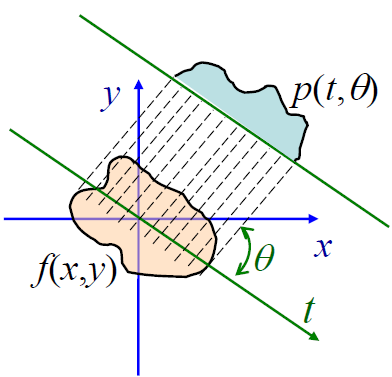
\includegraphics[scale=0.75]{Immagini/radon.png}
\caption{\label{fig:radon} \textit{Oggetto scansionato e sua proiezione}.}
\end{figure}

Dall'insieme delle proiezioni (trasformate di Radon) si ricava il \textbf{sinogramma}. Un sinogramma, mostrato nella \figref{fig:sino}, è un’immagine formata da sinusoidi, ad altezza fissata sul rivelatore, le cui righe rappresentano la proiezione lineare dell'oggetto all'angolo $\theta$; inoltre, deve essere simmetrico rispetto al centro di rotazione e rispetto a rotazioni di 180°. In realtà, l'antitrasformata di Radon vale solamente per variazioni continue di $\theta$, per questo motivo non può essere impiegata nella pratica, dove ovviamente è possibile avere solo variazioni discrete dell'angolo che definisce la direzione di scansione. Si usa, quindi, una versione discretizzata dell'antitrasfornata di Radon.

\begin{figure}[htp]
\centering
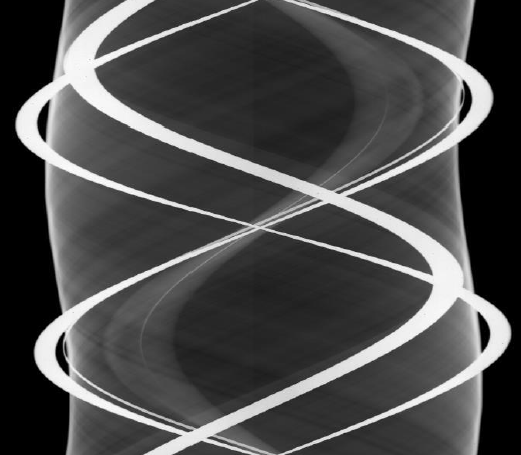
\includegraphics[scale=0.64]{Immagini/sinogramma.png}\quad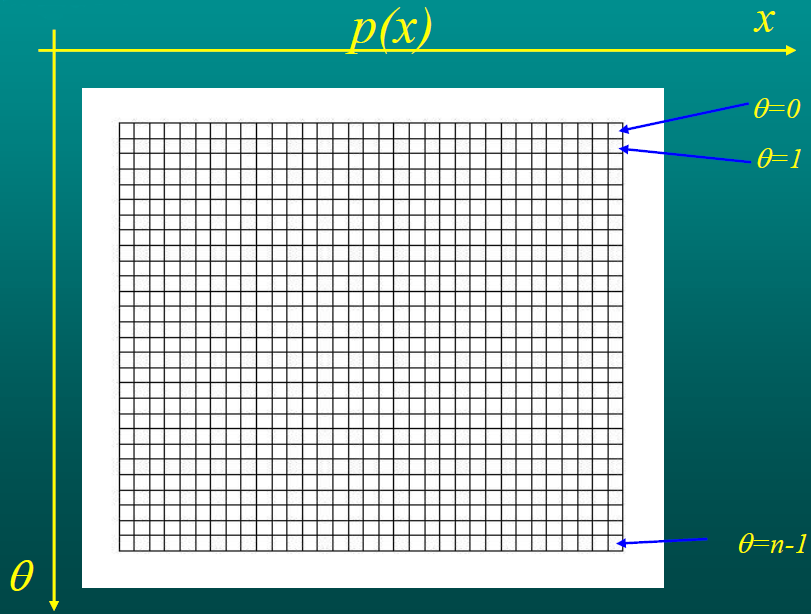
\includegraphics[scale=0.38]{Immagini/sino.png}
\caption{\label{fig:sino} \textit{Sinogramma di un globo e piano di riempimento di un sinogramma}.}
\end{figure}

Una volta che si è acquisito il sinogramma, prima di applicare l'antitrasformata di Radon, per migliorare la qualità dell'immagine (ad esempio rimuovendo rumore o artefatti) è opportuno passare allo spazio delle frequenze. Lo spazio delle frequenze, o spazio di Fourier (\figref{fig:frequenze}), si ottiene applicando al sinogramma la trasformata di Fourier. Se ad ogni proiezione acquisita si applica la trasformata di Fourier, si ottiene una serie di linee nel dominio delle frequenze; tali linee hanno, nel dominio delle frequenze, lo stesso angolo dell'asse \textit{t} corrispondente nello spazio (\textit{x,y}). Questa operazione è conveniente in quanto è molto più semplice operare nello spazio di Fourier per migliorare la qualità dell'immagine, rispetto a quanto non lo sia nello spazio reale utilizzando i \textit{kernel}, come spiegato prima. Una volta che si è migliorata la qualità dell'immagine, si applica l'antitrasformata di Fourier per tornare al sinogramma, e da lì si applica l'antitrasformata di Radon per ottenere l'oggetto.

\begin{figure}[htp]
\centering
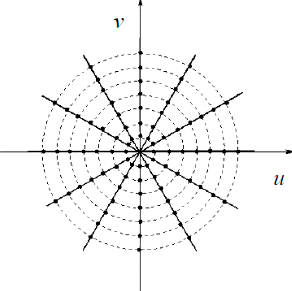
\includegraphics[scale=0.84]{Immagini/frequenze.png}
\caption{\label{fig:frequenze} \textit{Dominio delle frequenze o spazio di Fourier}.}
\end{figure}

L'applicazione dell'antitrasformata di Radon costituisce il processo di \textit{back projection} o retroproiezione. Per capire di cosa si tratta, prendiamo una matrice $3\times3$ di numeri che rappresentano un'immagine, e consideriamo 4 proiezioni, come mostrato nella \figref{fig:proiezione}. Ogni valore proiettato lungo una linea è dato dalla somma dei valori di ciascuna casella della matrice per i quali quella stessa linea passa: questo processo di proiezione è detto \textit{forward projection} e viene eseguito dallo scanner TC in fase di acquisizione. La retroproiezione è il procedimento opposto, in cui lo scanner deve risalire, a partire dalle proiezioni che ha acquisito, al contenuto di ciascuna casella della matrice, che di solito per un'immagine TC è in formato $512\times512$. Nella sua versione più semplice, la retroproiezione viene eseguita semplicemente spalmando il valore delle proiezioni lungo ciascuna linea; tuttavia, questo metodo fornisce risultati non soddisfacenti, in particolare immagini soggette a una caratteristica sfocatura inversamente proporzionale alla distanza dal centro dell'immagine stessa. Per evitare la sfocatura, tra i processi di \textit{forward projection} e \textit{back projection} è necessario filtrare, nello spazio di Fourier, le frequenze che causano la sfocatura e, più in generale, che abbassano la qualità dell'immagine; con questa aggiunta, il processo di retroproiezione prende il nome di \textit{filtered back projection} (FBP). L'impiego delle trasformate e antitraformate di Radon e Fourier è proprio un metodo di FBP.

\begin{figure}[htp]
\centering
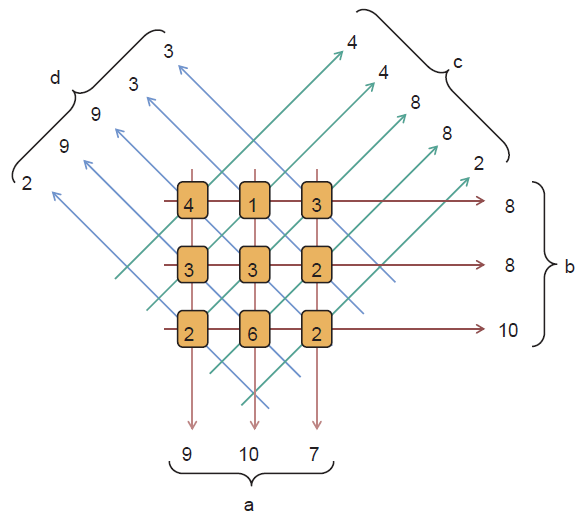
\includegraphics[scale=0.65]{Immagini/proiezione.png}
\caption{\label{fig:proiezione} \textit{Esempio di forward projection per una matrice $3\times3$. Fonte:} \cite[352]{bushberg}.}
\end{figure}

\section{Segmentazione}
Segmentare un’immagine significa riconoscere al suo interno elementi con caratteristiche in comune, distinguere questi elementi da altri con caratteristiche diverse e raggruppare tutti gli elementi simili in regioni, delineando dei bordi tra di esse. In un’immagine digitale, la segmentazione consiste nel classificare e quantificare in qualche modo le proprietà di ciascun pixel, come l’intensità per le immagini monocromatiche, il colore e la \textit{texture}.

Sia \textit{R} l’intera regione di spazio occupata da un’immagine. Possiamo definire la segmentazione di un’immagine come il processo che porta a dividere \textit{R} in sottoregioni $R_i$, con $i = 1,\,\dots,\,n $ tale che:
\begin{enumerate}
\item $\bigcup\limits_{i=1}^n R_i = R$;
\item $R_i$ è un insieme connesso per $i = 1,\,\dots,\,n$;
\item $R_i \cap R_j = \varnothing$;
\item $ \text{Q}(R_k) = 1 $;
\item $ \text{Q}(R_k \cup R_j) = 0 $ per ogni coppia di regioni adiacenti $R_k$ e $R_j$;
\end{enumerate}
dove $\text{Q}(R_k)$ è un predicato logico definito per i punti appartenenti a $R_k$. La condizione 1. asserisce che la segmentazione debba essere completa, nel senso che ogni pixel debba essere incluso in una sottoregione. La condizione 2. richiede che le sottoregioni siano connesse, cioè che non sia possibile individuare al loro interno due o più insiemi aperti, non vuoti e disgiunti. La condizione 3. richiede che le stesse sottoregioni siano disgiunte. La condizione 4. definisce l’assegnazione di un valore booleano a ciascuna sottoregione in base al soddisfacimento di proprietà da definire. Infine, la condizione 5. indica che due sottoregioni adiacenti debbano essere differenti per almeno una proprietà \cite[700]{gonzalez}.

In campo medico, la segmentazione è impiegata per studiare strutture anatomiche, identificare regioni d’interesse dove sono localizzati tumori o lesioni e, cosa più importante per l’obiettivo di questa tesi, misurare il volume dei tessuti corporei. Attualmente nella maggior parte delle strutture sanitarie la segmentazione è effettuata manualmente da un radiologo/radioterapista. La segmentazione manuale dei tessuti corporei è un processo ripetitivo, dispendioso in termini di tempo ed operatore-dipendente: di conseguenza non viene svolto con regolarità su tutte le immagini TC acquisite dai pazienti, sebbene farlo porterebbe a numerosi vantaggi in diversi ambiti. In parecchie strutture, comunque, la segmentazione dei tessuti corporei viene eseguita anche mediante software di segmentazione semiautomatica: si tratta di software che propongono una segmentazione dell'immagine, la quale però necessita di essere comunque controllata e corretta manualmente da un radiologo. Le implicazioni e i vantaggi della segmentazione automatica vengono ampiamente discusse nei capitoli successivi.

Tornando alle basi teoriche della segmentazione, il metodo più semplice è il \textit{thresholding}, in italiano sogliatura, fondato sull'assunto che regioni differenti di un’immagine siano caratterizzate da diversi valori d’intensità. Questo metodo si fonda sul trovare un valore soglia di grigio (\textit{threshold}) tale per cui se un pixel supera quel valore viene considerato un pixel oggetto (\textit{foreground}), mentre se non lo supera viene classificato come pixel di sfondo (\textit{background}) \cite[743]{gonzalez}. Il \textit{thresholding} funziona bene quando sono presenti solo due classi di pixel e se tutti i pixel all’interno di ogni classe hanno intensità simili \cite[20]{LaRosa}; in caso contrario, il metodo da implementare dovrà essere il \textit{multithresholding}, che si fonda sugli stessi principi del \textit{thresholding} ma prevede più di una classe di intensità. Uno dei metodi più famosi di sogliatura è il \textit{thresholding} di Otsu, un algoritmo che trova automaticamente il \textit{threshold}, calcolandolo in modo tale da minimizzare la varianza all'interno di una stessa classe o, equivalentemente, massimizzare la varianza tra le classi. Il metodo di Otsu richiede soltanto l'istogramma di un immagine, ma presenta diverse limitazioni quando il \textit{foreground} e il \textit{background} sono caratterizzati da intensità medie vicine e varianza elevata al loro interno \cite[20]{LaRosa}.

Oltre al \textit{thresholding}, gli algoritmi di segmentazione per immagini monocromatiche funzionano in base a una delle due seguenti proprietà: discontinuità e similarità. L’approccio più comunemente usato per la prima categoria è la segmentazione \textit{edge based}, la quale per funzionare bene necessita che i bordi delle regioni siano sufficientemente diversi l’uno dall'altro e dallo sfondo, in modo da permettere un riconoscimento dei bordi basato sulle discontinuità di intensità locali \cite[700]{gonzalez}. La seconda categoria sfrutta invece la segmentazione \textit{region based}, che consiste nel raccogliere in un gruppo, il \textit{cluster}, pixel con proprietà sufficientemente simili da formare insieme una regione omogenea; il criterio di omogeneità è determinato di solito dal livello di grigio dei pixel \cite{Sharma2010}.

\section{Reti neurali} \label{retineurali}
I recenti software di segmentazione automatica si fondano sul \textit{deep learning}, una branca del \textit{machine learning} basata su reti neurali di algoritmi e che si occupa dei metodi di autoapprendimento per lo svolgimento di compiti complessi. Ciò è possibile grazie alla creazione, in automatico da parte della macchina, di modelli statistici gerarchici, costruiti a partire dalle informazioni più semplici per arrivare alle rappresentazioni più complesse. Ciascuna informazione contenuta in una rappresentazione è chiamata \textit{feature}, o caratteristica; le \textit{feature} create da un umano e fornite alla macchina sono dette \textit{hand crafted feature} \cite[11]{LaRosa}. Più precisamente, una \textit{feature} è una proprietà individuale e misurabile di un fenomeno osservato \cite{bishop, wiki:feature}, solitamente resa in forma numerica \cite{wiki:feature}. Un'importante caratteristica delle reti di \textit{deep learning} è che esse sono costituite da una serie di \textit{layer} successivi: ad ogni \textit{layer}, il segnale in input viene processato e passato al \textit{layer} successivo. I \textit{layer} che si trovano fra l'input e l'output sono definiti nascosti e una rete che abbia questa struttura viene chiamata rete neurale \cite[12]{LaRosa}.

Le reti neurali utilizzate per realizzare gli studi presentati nei capitoli successivi seguono tutte un unico paradigma di apprendimento, l'apprendimento supervisionato. Si tratta di fornire alla rete un insieme di dati di addestramento (\textit{training set}) costituito da oggetti di input e dagli output desiderati, in modo che la rete possa estrarre \textit{feature} significative e trovare una relazione fra l'input e l'output. Successivamente vengono aggiustati i pesi e altri parametri della rete in maniera tale da minimizzare l'errore di previsione relativo al \textit{training set}. Alla fine dell'addestramento, la rete dovrebbe essere in grado di fare delle previsioni, su dati diversi da quelli del \textit{training set}, sull'output desiderato quando questo non è noto a priori \cite{wiki:rete}.

Le reti neurali a convoluzione (CNN), ampiamente utilizzate nei software di segmentazione automatica dei tessuti corporei, sono un tipo di reti neurali artificiali ispirate alla corteccia visuale degli organismi animali, in cui i neuroni sono organizzati in modo da essere sensibili solo a una piccola sottoregione del campo visuale, detta campo ricettivo; i campi ricettivi di tutti i neuroni messi insieme coprono tutto il campo visuale. La convoluzione è la principale operazione matematica impiegata nelle CNN \cite[12]{LaRosa}. La differenza sostanziale fra le CNN e le altre reti neurali artificiali sta nell'organizzazione \virgolette{a griglia} dei dati in input; per questo motivo, le CNN funzionano particolarmente bene quando i dati in input sono delle immagini, che possono essere viste come griglie bidimensionali di pixel. Una qualsiasi CNN è composta da diversi \textit{convolutional} e (eventuali) \textit{pooling layer} alternati, seguiti da uno o più \textit{fully connected layer} prima dell'output. Semplificando, i \textit{convolutional layer} servono ad aumentare le dimensioni dei dati, eseguendo convoluzioni fra un filtro e le immagini 2D: il risultato sarà una mappa d'attivazione per ogni immagine 2D, e tutte le mappe vengono unite insieme per generare un output tridimensionale \cite[13]{LaRosa}. I \textit{pooling layer}, al contrario, servono ad abbassare la dimensione degli input che giungono loro dai \textit{convolutional layer}, prendendo da ciascuna \textit{slice} $2\times2$ soltanto il valore più alto (\textit{max pooling}) o il valore medio (\textit{average pooling}), e mandando questi valori in input al \textit{convolutional layer} successivo \cite{wiki:CNN}. Infine, i \textit{fully connected layer} connettono ogni neurone in un \textit{layer} con ogni neurone in un altro \textit{layer} \cite{wiki:CNN}.

Senza scendere troppo nei particolari della struttura delle CNN, in sostanza queste reti prendono in input un'immagine e restituiscono in output un vettore contenente le probabilità dell'immagine di appartenere a ogni classe prevista: in base a questo, una CNN può essere facilmente adattata per segmentare delle immagini, dove ciascun pixel verrà assegnato a una classe \cite[23]{LaRosa}. Per ridurre il numero di calcoli, il \textit{fully connected layer} può essere sostituito con delle convoluzioni, ma in questo modo l'output della rete risulta di dimensione inferiore all'input; per ovviare a questo problema si possono usare delle operazioni di deconvoluzione, per aumentare la dimensione dell'output fino a che questa abbia raggiunto la stessa dimensione dell'input. Una CNN che non prevede \textit{fully connected layer} nella sua struttura è definita \textit{fully convolutional network} \cite[23-24]{LaRosa}, di cui un importante esempio, nell'ambito della segmentazione automatica, sono le U-Net, chiamate così per la forma a \virgolette{U} che assume la loro schematizzazione, riportata nella \figref{fig:unet}. Il ramo discendente, detto percorso di contrazione (\textit{contracting path}) consiste di due applicazioni ripetute di convoluzioni $3\times3$ e di una operazione di \textit{max pooling} $2\times2$: a ogni \textit{layer}, quindi, la dimensione dell'immagine si dimezza, perdendo informazione spaziale ma aumentando l'informazione sulle \textit{feature}. Al contrario, lungo il ramo ascendente, detto percorso di espansione (\textit{expanding path}), le due applicazioni di convoluzioni $3\times3$ sono seguite da una deconvoluzione $2\times2$, in modo che la dimensione dell'immagine raddoppi a ogni \textit{layer} successivo \cite{wiki:unet}. In questo modo si riacquista l'informazione spaziale persa durante il percorso di contrazione e la si combina con l'informazione sulle \textit{feature} acquisita sempre durate il percorso di contrazione.

\begin{figure}[htp]
\centering
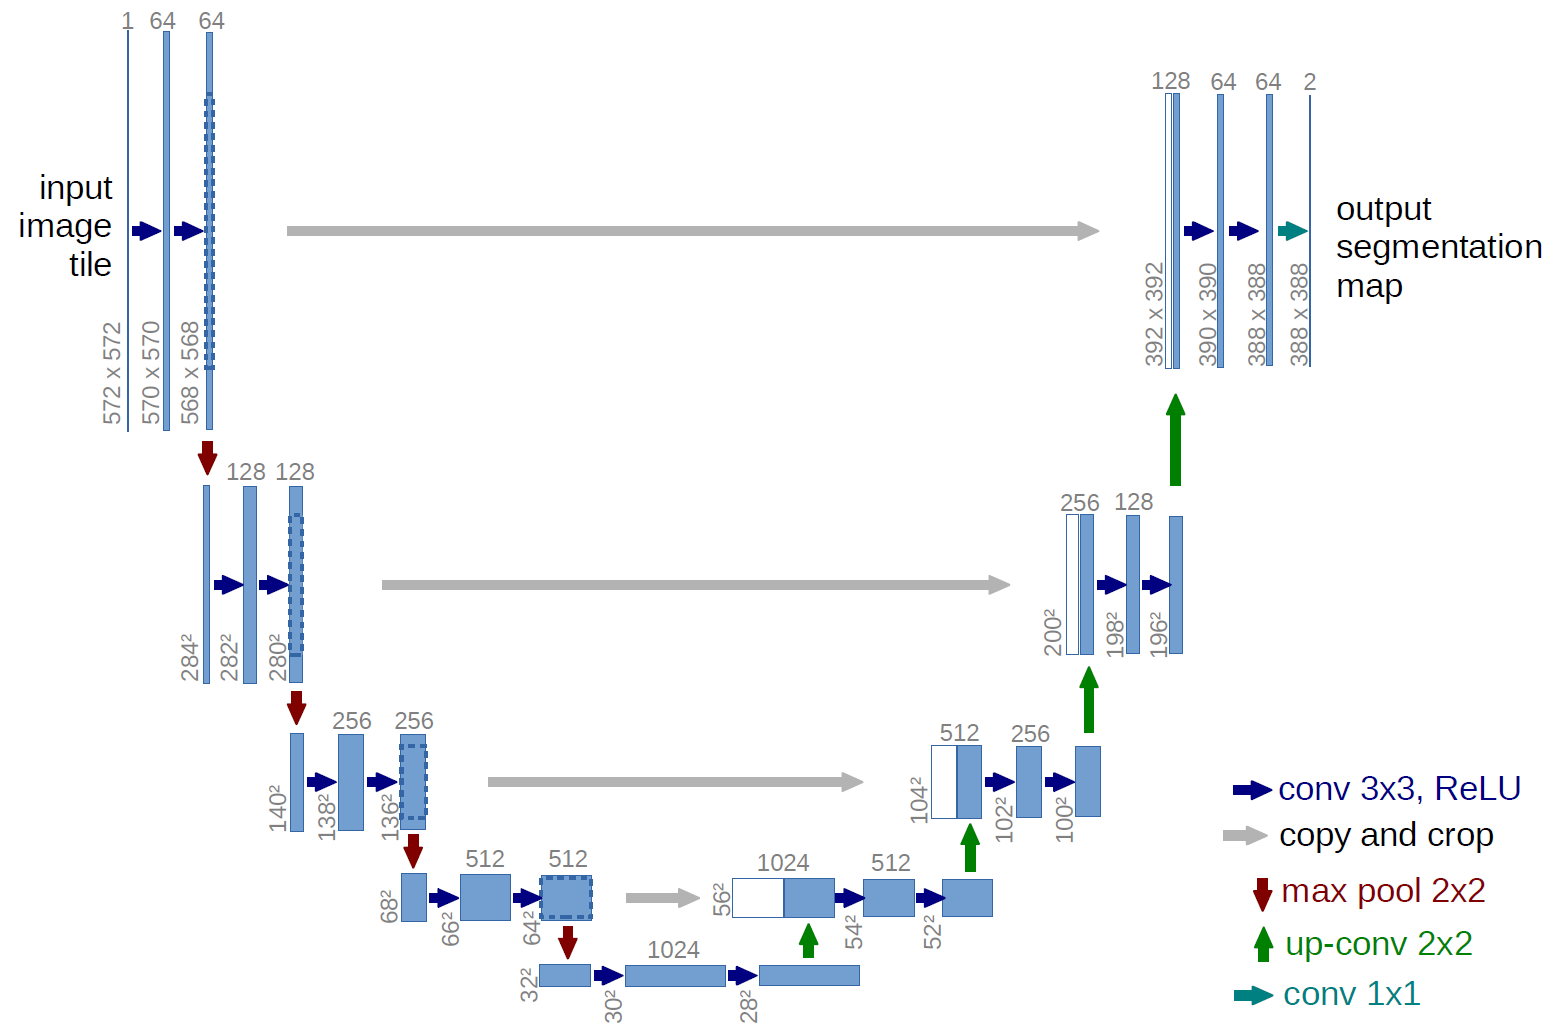
\includegraphics[scale=0.25]{Immagini/unet.png}
\caption{\label{fig:unet} \textit{Schematizzazione di una U-Net}.}
\end{figure}

\section{Metodi statistici per la valutazione della stima della \textit{body composition}}

\subsection{Metodo Kaplan-Meier}\label{km}
In medicina, nei test clinici o comunitari di un determinato farmaco o trattamento, gli effetti della terapia da studiare vengono valutati misurando il numero di soggetti sopravvissuti per un certo periodo di tempo che sono stati sottoposti a quella terapia. Analisi di questo tipo si rivelano spesso complicate per diverse cause: \textit{in primis} alcuni soggetti potrebbero morire durante la finestra di tempo in cui si colloca lo studio ma per cause diverse da quelle studiate, mentre altri ancora non cooperano o smettono di fornire informazioni ai medici sul proprio stato di salute. Per tutti i pazienti per i quali si hanno informazioni parziali si dice che il tempo di sopravvivenza è troncato a destra (\textit{right censored}). Possono esserci anche altri pazienti che si uniscono allo studio dopo il suo inizio, per i quali quindi si ha un tempo di osservazione più breve. Se si vuole tenere conto di tutte queste situazioni, il metodo più semplice è quello di Kaplan-Meier \cite{Goel2010}.

La curva di sopravvivenza di Kaplan-Meier è definita come la probabilità di sopravvivenza in un determinato periodo di tempo, il tempo di sopravvivenza o \textit{serial time}, suddiviso in intervalli più piccoli \cite{altman, Goel2010}. La durata del tempo di sopravvivenza nota di un soggetto è determinata dal verificarsi di un evento di interesse, sia esso la morte del paziente o un altro evento; questo periodo di tempo è noto con il nome di intervallo nell'analisi di Kaplan-Meier ed è rappresentato con una linea orizzontale, come mostrato nella \figref{fig:mm_kaplanmeier}. In altre parole, solo il verificarsi dell'evento di interesse definisce la sopravvivenza nota, mentre i soggetti censurati, rappresentati nella \figref{fig:mm_kaplanmeier} con delle croci, non terminano l'intervallo e quindi non sono associati a nessuno \virgolette{scalino} nel diagramma \cite{Rich2010}. L'analisi di Kaplan-Meier presuppone tre assunzioni:
\begin{itemize}[label=$-$]
    \item ad un qualsiasi istante di tempo i soggetti censurati hanno la stessa aspettative di sopravvivenza dei soggetti di cui si continua ad avere informazioni;
    \item le probabilità di sopravvivenza sono le stesse per tutti i soggetti, a prescindere da quando essi siano stati inclusi nello studio;
    \item qualsiasi evento avviene in un preciso istante di tempo (per eventi su cui si ha incertezza riguardo all'istante di avvenimento, fa fede l'istante al quale l'avvenimento è stato scoperto).
\end{itemize}
Chiaramente, maggiore è la frequenza con la quale vengono acquisite informazioni dai pazienti (sia che riguardino la morte del paziente, sia che riguardino il verificarsi di un evento specifico), maggiore sarà anche l'accuratezza della stima \cite{Goel2010}.

\begin{figure}[htpb]
\centering
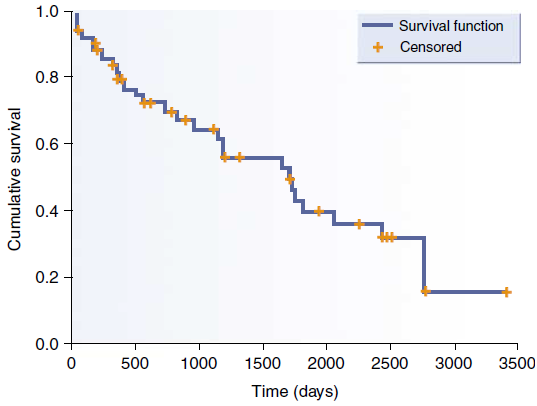
\includegraphics[scale=0.89]{Immagini/mm_kaplanmeier.png}
\caption{\label{fig:mm_kaplanmeier} \textit{Diagramma di Kaplan-Meier della sopravvivenza. Fonte:} \cite{Jager2008}.}
\end{figure}

La sopravvivenza cumulativa mostrata nella \figref{fig:mm_kaplanmeier} è così calcolata: ogni volta che un soggetto X muore, per calcolare la sopravvivenza cumulativa dell'intervallo successivo si prende la frazione di soggetti rimasti in vita subito dopo la morte del soggetto X e la si moltiplica per la sopravvivenza cumulativa dello step precedente, ossia un istante prima che il soggetto X morisse. Si ripete il processo ogni volta che si verifica la morte di un soggetto fino alla fine del periodo di raccolta dati, momento in cui tutti i pazienti rimasti in vita vengono censurati; da questo momento in poi non si hanno più informazioni sui pazienti rimasti in vita, e ognuno di questi potrebbe sopravvivere per diversi anni dopo la fine dell'osservazione con la stessa probabilità con cui potrebbe sopravvivere solo alcune ore, ragion per cui l'estrapolazione dei dati oltre il periodo di osservazione non è giustificata \cite{Rich2010}.

Esistono diversi tipi di curve di sopravvivenza, che si differenziano principalmente per gli eventi d'interesse. Nelle curve di sopravvivenza generale (\textit{overall survival}) l'evento d'interesse è la morte del soggetto per qualsiasi causa, il che fa attribuisce a questo tipo di curva un significato di mortalità piuttosto generale. Nelle curve di \textit{disease free survival} l'evento di interesse è la recidiva di una malattia, mentre le curve di \textit{progression free survival} usano la progressione di una malattia (ad esempio la diffusione di un tumore) come punto finale di un intervallo della curva. Infine, nelle curve di sopravvivenza da malattie specifiche (\textit{disease specific survival}) l'evento di interesse è la morte del soggetto come conseguenza di una malattia specifica; questo tipo di curva può portare a volte a risultati distorti, poiché sarà sempre più alta di curve come quelle di \textit{overall survival} e \textit{disease free survival}, in quanto gli eventi d'interesse sono limitati a una sola malattia specifica \cite{Rich2010}.

\subsection{Modelli di comparazione}\label{confronto}
Un punto importante che rimane da discutere è la comparazione di due curve di sopravvivenza, che torna utile, ad esempio, se si vuole valutare la significatività statistica della differenza fra due curve rappresentanti lo stesso fenomeno ma con cause diverse: ad esempio, la morte di soggetti a causa di insufficienza renale cronica terminale (ESRD) dovuta al diabete o ad altre cause, il cui diagramma di Kaplan-Meier è riportato nella \figref{fig:mm_kaplanmeier2}.

\begin{figure}[htp]
\centering
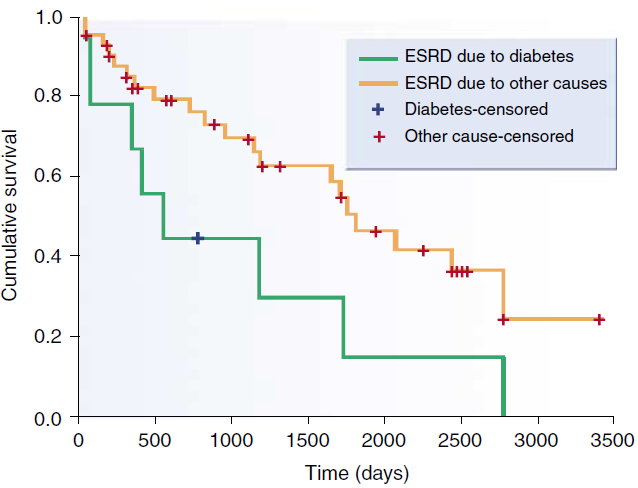
\includegraphics[scale=0.78]{Immagini/mm_kaplanmeier2.png}
\caption{\label{fig:mm_kaplanmeier2} \textit{Diagramma di Kaplan-Meier della sopravvivenza di soggetti estratti da un gruppo a rischio di morte per ESRD dovuta a diabete o ad altre cause. Fonte:} \cite{Jager2008}.}
\end{figure}

Il metodo più comune di comparazione tra due curve di sopravvivenza è il \textit{log-rank test}, che calcola il valore del \textit{chi} quadrato per ogni intervallo di ciascuna curva e li somma tra di loro. Prese due curve di sopravvivenza, siano $E_1$ e $E_2$ i valori di aspettazione del numero di eventi in ciascun gruppo, e siano $O_1$ e $O_2$ il numero totale di eventi osservati in ciascun gruppo. Il \textit{chi} quadrato sarà definito come segue:
\begin{equation}
    \chi^2 = \frac{(O_1-E_1)^2}{E_1} + \frac{(O_2-E_2)^2}{E_2}\,.
\end{equation}
Supponiamo di voler calcolare il valore di aspettazione $E_2$ del numero di eventi del gruppo 2 in un dato intervallo di tempo; questo sarà dato dal prodotto della probabilità dell'evento in entrambi i gruppi 1 e 2 in quell'intervallo (in pratica, la frazione di persone morte dall'inizio alla fine dell'intervallo in entrambe i gruppi) e del numero di persone vive all'inizio dell'intervallo nel solo gruppo 2. Eseguendo questo prodotto per ciascun intervallo del gruppo 2, troviamo il valore di aspettazione totale del gruppo 2. Per trovare il valore di aspettazione totale del gruppo 1, è sufficiente sottrarre al totale degli eventi osservati il valore di aspettazione del gruppo 2 \cite{Goel2010}:
\begin{equation}
    E_1 = (O_1+O_2)-E_2\,.
\end{equation}
Dopo aver ottenuto il $\chi^2$, si controlla il \textit{p-value} all'interno della tavola del \textit{chi} quadrato per un solo grado di libertà e si stabilisce la significatività della differenza fra i due gruppi se il \textit{p-value} è minore di un certo valore stabilito a priori.

Il \textit{log-rank test} permette unicamente di stabilire la significatività statistica della differenza fra le curve di sopravvivenza di due gruppi, perciò è utile solo in analisi univariate. Per lo svolgimento di analisi multivariate nel campo delle curve di sopravvivenza, il metodo più diffuso è il modello di regressione di Cox (\textit{Cox proportional hazards model}), che permette di testare l'effetto di altre variabili indipendenti sui tempi di sopravvivenza dei diversi gruppi \cite{Goel2010}, ad esempio per lo studio del rapporto tra un fattore di rischio (come il fumo) e l’incidenza di un determinato esito clinico (come l'infarto del miocardio), correggendo per uno o più fattori di confondimento (quali l’obesità e l’ipertensione) \cite{Provenzano2013}. Il rischio (\textit{hazard}) costituisce la variabile dipendente ed è definito come la probabilità di morte ad un certo istante \cite{Goel2010}; in altre parole, è il tasso di incidenza di un evento d'interesse, cioè il numero di eventi per persona per unità di tempo \cite{Provenzano2013}. Il rapporto di rischio, invece, è il rapporto tra i tassi di rischio istantanei di un evento d'interesse in due gruppi diversi \cite{wiki:rischio}: per fare un esempio, se $H_1,\,H_2,\,H_3,\,\dots$ e $h_1,\,h_2,\,h_3,\,\dots$ sono i tassi di rischio per due gruppi agli istanti $T_1,\,T_2,\,T_3,\,\dots$, i rapporti di rischio agli istanti $T_1,\,T_2,\,T_3,\,\dots$ saranno rispettivamente $\frac{H_1}{h_1},\,\frac{H_2}{h_2},\,\frac{H_3}{h_3}\,,\dots$. Si assume che il tasso di rischio rimanga costante nel tempo, ossia che $\frac{H_1}{h_1}=\frac{H_2}{h_2}=\frac{H_3}{h_3}=\dots$ \cite{Goel2010}.

L’equazione generale di un modello di regressione di Cox avente
l’obiettivo di analizzare il rapporto tra la presenza/assenza di un singolo
fattore di rischio e un determinato esito clinico è la seguente:
\begin{equation}\label{rischio}
    h_i(t) = \lambda_0(t)\,\mathrm{e}^{\beta_1 x_i}\,,
\end{equation}
dove $h_i(t)$ è il tasso di incidenza stimato dell'evento al tempo \textit{t}, $\lambda_0(t)$ rappresenta il rischio di base, cioè il tasso di incidenza dell'evento in assenza del fattore di rischio, $\beta_1$ è il coefficiente di regressione e $x_i$ è il fattore di rischio considerato. Applicando il logaritmo naturale all'\eqref{rischio}, si ottiene:
\begin{equation}
    \ln{(h_i(t))} = \ln{(\lambda_0(t))} + \beta_1 x_i = \beta_0(t) + \beta_1 x_i\,;
\end{equation}
in questa forma, l'equazione sembra più simile a una classica equazione di regressione lineare \cite{Goel2010, vanDijk2008}.

\subsection{Metodo Bland-Altman}\label{blandaltman}
I metodi di correlazione sono strumenti statistici che rivelano in che misura delle coppie di variabili sono correlate. Il risultato principale di una correlazione è il coefficiente di correlazione \textit{r}, che può variare da $-1$ a $+1$, e più si avvicina agli estremi, più le variabili saranno correlate. Tuttavia, le tecniche di correlazione descrivono solamente la relazione fra due insiemi di dati, non il loro accordo \cite{Udovicic2007,Giavarina2015}, risultando a volte inadeguate e foriere di risultati ambigui.

Il metodo Bland-Altman è uno strumento molto efficace per la valutazione dell'accordo fra due metodi di misurazione, consentendo inoltre di individuare la presenza di differenza sistematiche, valori anomali (\textit{outlier}) e particolari strutture di disaccordo (\textit{pattern}) \cite[357]{szklo,Franco2017}. In breve, il metodo quantifica il livello di accordo tra due misure mediante la definizione di due limiti di concordanza mostrati su uno \textit{scatter plot}: sull'asse delle ordinate viene posta la differenza fra due misure in una stessa coppia (che possono essere, ad esempio, due misure di pressione arteriosa effettuate su uno stesso soggetto con due metodi diversi), mentre sull'asse delle ascisse è riportato il valore medio delle due misure in una stessa. In un diagramma di Bland-Altman, di cui si riporta un esempio nella \figref{fig:ba}, sono presenti due elementi fondamentali:
\begin{itemize}[label=$-$]
    \item il \textit{bias}, cioè una linea appresentante la media delle differenze delle due misurazioni;
    \item i limiti di concordanza, due linee che vengono tracciate ad altezza $bias\,\pm\,1,96\,\sigma$, dove $\sigma$ è la deviazione standard.
\end{itemize}

Nel caso in cui la prima e la seconda misurazione fossero coincidenti, la media delle differenze sarebbe nulla e i punti sarebbero allineati lungo l’asse delle ascisse sul valore 0. La scelta di rappresentare in ascissa la media delle due misurazioni, al posto dei valori di una sola delle due misurazioni, si basa sul fatto di non conoscere a priori il valore vero della variabile in
esame; di conseguenza, si prende in considerazione la migliore stima, che è rappresentata dalla media \cite{Franco2017}.

Il valore di $1,96\,\sigma$ rispetto alla media (spesso approssimato a $2\,\sigma$) utilizzato come limite di concordanza è dovuto al fatto che, se le differenze fra le misure sono distribuite normalmente, queste devono essere contenute per il 95\% del totale tra i due limiti così definiti. Non è necessario che le misure seguano una distribuzione normale \cite{BlandAltman}, mentre se le differenze non seguono una distribuzione normale, si può provare ad eseguire una trasformazione logaritmica dei dati originali per provare a normalizzare la distribuzione delle differenze \cite{Giavarina2015}.

Infine, per valutare se i dati forniti dai due metodi di misura abbiano un livello di accordo sufficiente, l'unico modo è confrontarli con limiti di accettabilità definiti a priori in base a criteri clinici e analitici: se i limiti di concordanza trovati con l'analisi di Bland-Altman cadono all'interno dei limiti di accettabilità, allora consideriamo i due insiemi di dati sufficientemente concordi \cite{Giavarina2015}. Nel caso si confrontino un metodo di misura \textit{gold standard} e un metodo di misura, una buona regola pratica è quella di considerare come \textit{bias} accettabile un valore non superiore del 3-4\% rispetto a quello fornito dal dispositivo \textit{gold standard} \cite{Weinfurt2010,Franco2017}.

\begin{figure}[htp]
\centering
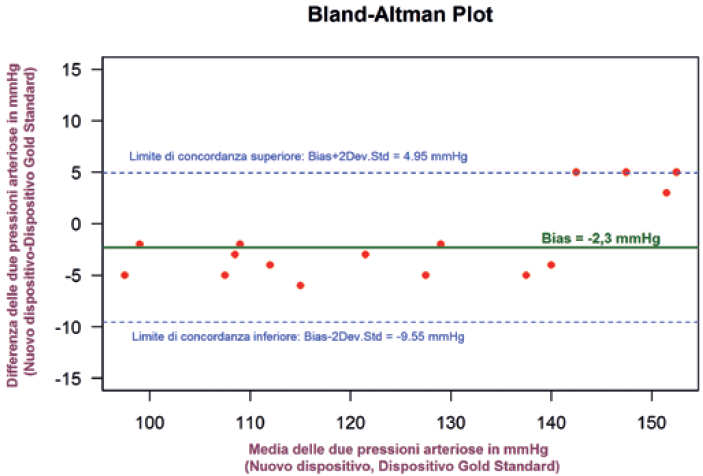
\includegraphics[scale=0.8]{Immagini/ba.png}
\caption{\label{fig:ba} \textit{Grafico di Bland-Altman dell'accordo nelle misurazioni della pressione diastolica con due dispositivi: il gold standard e il nuovo
dispositivo. Si può notare che per valori di pressione media superiori a $140\,\mathrm{mmHg}$ il nuovo dispositivo fornisce misure non concordanti con quelle del gold standard. Fonte:} \cite{Franco2017}.}
\end{figure}
\clearpage
\null
\newpage
\chapter{Obiettivi clinici dello studio della composizione del corpo}\label{capitolo2}
La TC, soprattutto nella regione addominale, è una tipologia di indagine molto diffusa per un’ampissima gamma di situazioni. Oltre allo scopo principale per cui una TC viene prescritta, che varia a seconda del caso, questa può essere utilizzata per ottenere una grande quantità di informazioni aggiuntive su fattori di rischio o altre patologie: l’approccio per cui vengono processate anche queste informazioni secondarie è chiamato di \textit{screening} opportunistico. Nel presente capitolo vengono presentati i vantaggi di questo approccio sotto diversi punti di vista, mediante alcuni studi che evidenziano la parziale inadeguatezza dei protocolli attualmente utilizzati in fase di valutazione della composizione corporea dei pazienti.

\section{Osteoporosi}
Uno degli obiettivi che può essere perseguito con lo \textit{screening} opportunistico è la valutazione della densità ossea, che se diventa troppo bassa configura una condizione clinica nota come osteoporosi, molto diffusa fra i pazienti, soprattutto donne, in età avanzata. L’età rappresenta infatti il maggior fattore di rischio, che però può essere contrastato riducendo altri fattori di rischio, come fumo di sigaretta, abuso di alcol e dieta carente di minerali essenziali. Se si scopre una densità ossea troppo bassa a seguito di uno \textit{screening} è possibile intervenire per tempo per evitare o ritardare l’insorgenza della malattia. La tecnica ad oggi più utilizzata per stimare la densità delle ossa è la densitometria ossea a raggi X a doppia energia, abbreviata in DXA: questa tecnica comporta la misurazione dell'attenuazione di due fasci di raggi X di diversa energia, in modo da poter derivare la densità (per unità di superficie, trattandosi di un'indagine che fornisce immagini bidimensionali) di un materiale in presenza di un altro a partire dalle diverse attenuazioni dei due materiali per energie diverse. Una volta nota l'attenuazione, possiamo risolvere un sistema di due equazioni a due incognite, approssimando l’attenuazione reale come quella di un fascio monocromatico attraverso la legge di Lambert-Beer (\eqref{lambert}), la quale può essere riscritta nel seguente modo:
\begin{equation}
    I = I_0\,\mathrm{e}^{-\mu x} = I_0\,\mathrm{e}^{-\left(\frac{\mu}{\rho}\right) \rho x} = I_0\,\mathrm{e}^{-\left(\frac{\mu}{\rho}\right) \sigma}\,,
\end{equation}
dove $\frac{\mu}{\rho}$ rappresenta il coefficiente di attenuazione di massa, i cui valori sono tabulati e dipendono dal materiale e dall'energia del fascio, e $\sigma$ è la densità di massa superficiale. Le due equazioni per i due fasci a energia differente sono:
    \[
\begin{sistema} 
I^\mathrm{L} = I_0\,\mathrm{e}^{- \left[ \left(\frac{\mu}{\rho}\right)^\mathrm{L}_\mathrm{s} \sigma_\mathrm{s} + \left(\frac{\mu}{\rho}\right)^\mathrm{L}_\mathrm{b} \sigma_\mathrm{b} \right]} \\
I^\mathrm{H} = I_0\,\mathrm{e}^{- \left[ \left(\frac{\mu}{\rho}\right)^\mathrm{H}_\mathrm{s} \sigma_\mathrm{s} + \left(\frac{\mu}{\rho}\right)^\mathrm{H}_\mathrm{b} \sigma_\mathrm{b} \right]}
\end{sistema}\,,
    \]
dove gli apici H e L indicano l'energia (alta o bassa) del fascio, mentre pedici s e b indicano il tipo di tessuto (molle o osseo). Il sistema è risolto per:
\begin{equation}
    \sigma_\mathrm{b} = \dfrac{R_\mathrm{s} \ln{\left(\dfrac{I}{I_0}\right)^\mathrm{H}}- \ln{\left(\dfrac{I}{I_0}\right)^\mathrm{L}}}{\left(\dfrac{\mu}{\rho}\right)^\mathrm{L}_\mathrm{b} - \left(\dfrac{\mu}{\rho}\right)^\mathrm{H}_\mathrm{b} R_\mathrm{s}}\,,
\end{equation}
dove con $R_\mathrm{s}$ indichiamo:
\begin{equation}
    R_\mathrm{s} = \dfrac{\left(\dfrac{\mu}{\rho}\right)^\mathrm{L}_\mathrm{s}}{\left(\dfrac{\mu}{\rho}\right)^\mathrm{H}_\mathrm{s}}\,.
\end{equation}
$\sigma_\mathrm{s}$ si trova esattamente allo stesso modo \cite[17-22]{iaea}. Nell'ambito della DXA, l'esame si effettua sul segmento lombare della colonna vertebrale, sul femore o sul polso, a seconda dell'età e del sesso del paziente. La densità ossea misurata viene confrontata col valore medio di una popolazione di giovani adulti sani, calcolando lo scostamento dal valore di riferimento in termini di deviazioni standard; il numero di deviazioni standard dal riferimento è definito \textit{T-score}. In presenza di un \textit{T-score} maggiore di $-1$ la densità ossea è considerata normale, tra $-1$ e $-2,5$ si configura l'osteopenia, mentre per \textit{T-score} inferiori a $-2,5$ viene diagnosticata l'osteoporosi \cite{siommms}.

Alternativamente, il calcolo della densità ossea può anche essere eseguito con una tecnica nota come TC quantitativa (QCT), ponendo vicino al paziente un fantoccio di fosfato di potassio (\figref{fig:fantoccio}), usato come riferimento per effettuare confronti tra la densità delle ossa del paziente e quella del fantoccio stesso \cite{Murray2017}. Il confronto viene effettuato attraverso la scala Hounsfield, che quantifica il valore di grigio dei pixel in un’immagine radiografica in unità di Hounsfield (HU), definite come segue:

\begin{equation}
    \mathrm{HU}(x,y,z) = 1000\times\frac{\mu(x,y,z) - \upmu_\mathrm{w}}{\upmu_\mathrm{w} - \upmu_\mathrm{a}}\,,
\end{equation}
dove $\mu(x,y,z)$ è il coefficiente di attenuazione lineare medio per elemento di volume (voxel) di tessuto in posizione $(x,y,z)$, mentre $\upmu_\mathrm{w}$ e $\upmu_\mathrm{a}$ sono i coefficienti di attenuazione lineare rispettivamente dell'acqua e dell'aria. Per l’acqua HU si annulla, per l’aria, che ha coefficiente di attenuazione lineare circa uguale a 1, assume il valore $-1000$; per quanto riguarda i tessuti del corpo, si va da un intervallo compreso tra $-80$ e $-30$\,HU per la maggior parte dei tessuti adiposi a un massimo di 3095\,HU per le ossa nella maggior parte dei macchinari di TC \cite[324-325]{bushberg}. La scala Hounsfield è importante perché stabilisce un criterio univoco di quantificazione per i valori di intensità dei pixel dell'immagine, permettendo così di confrontare immagini acquisite da macchinari diversi.
\begin{figure}[htp]
\centering
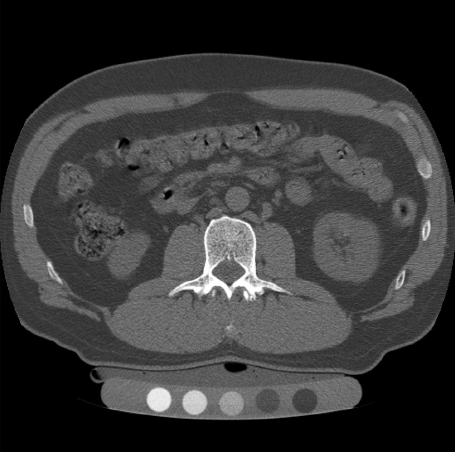
\includegraphics[scale=0.6505]{Immagini/fantoccio.png}\quad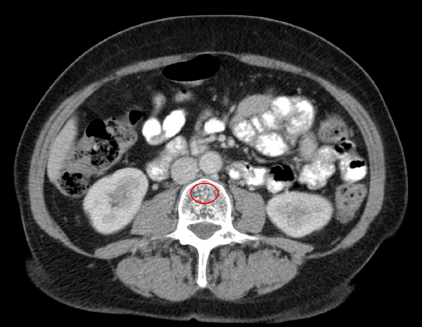
\includegraphics[scale=0.9]{Immagini/osteoporosi.png}
\caption{\label{fig:fantoccio} \textit{QCT eseguita con l'utilizzo di un fantoccio a diverse concentrazioni (immagine di sinistra) e CT addominale (L3), dove la vertebra presenta un valore di $106\,\mathrm{HU}$, compatibile con la diagnosi di osteoporosi (immagine di destra). Fonte:} \cite{wiki:fantoccio, Murray2017}.}
\end{figure}

Tornando alla QCT, questa ha un importante vantaggio rispetto alla DXA: trattandosi di un'indagine tomografica, questa misura la densità per unità di volume, al contrario delle misure della DXA che sono superficiali, ottenendo così dati riferiti al vero volume delle ossa. Valori di densità superiori ai $120\,\mathrm{mg}/\mathrm{cm}^3$ sono considerati normali, valori compresi tra 80 e $120\,\mathrm{mg}/\mathrm{cm}^3$ sono da considerarsi indicatori di osteopenia (una condizione di indebolimento delle ossa meno severa dell'osteoporosi), mentre per valori di densità inferiori a $80\,\mathrm{mg}/\mathrm{cm}^3$ si configura l’osteoporosi, di cui è possibile vedere un esempio nella \figref{fig:fantoccio}. Considerando una regione di interesse definita all'interno del corpo della vertebra, su una \textit{slice} trasversale a livello della vertebra L3, Murray \textit{et al.} riportano in uno studio \cite{Murray2017} che una soglia di 160\,HU raggiunge una sensibilità del 100\% e una specificità del 54\% per la diagnosi dell'osteoporosi, mentre la DXA si attesta su una sensibilità dell'88\% e una specificità del 62.5\% \cite{Humadi2010, Murray2017}. La specificità può essere migliorata ulteriormente fino al 63,8\% utilizzando delle tecniche più specifiche che tengano conto del grasso e dei muscoli paraspinali, responsabili di un abbassamento della densità nella regione d’interesse e, di conseguenza, di falsi positivi. Secondo un altro studio effettuato da Pickhardt \textit{et al.} \cite{Pickhardt2021}, sempre sulla QCT, misurazioni completamente automatiche dell'attenuazione all'altezza della vertebra L1 hanno dimostrato un buon accordo con i dati provenienti dalla selezione manuale della regione d’interesse.

Sebbene la QCT risulti essere molto più efficace, la DXA è attualmente lo standard nella valutazione della densità ossea; ciò avviene a causa dell'ancora limitata diffusione di metodi di segmentazione completamente automatici ma anche perché si tratta di un esame breve e che prevede l'utilizzo di dosi bassissime \cite{siommms}. In sintesi, la DXA fornisce risultati tutto sommato buoni ma sensibilmente peggiori rispetto a quelli di una TC, la quale andrebbe in ogni caso valutata e senza dubbio preferita all'interno di un approccio di \textit{screening} opportunistico, in quanto dimostra anche una migliore stratificazione dei pazienti a rischio frattura \cite{Pickhardt2021}.

\section{Obesità}
Come l’osteoporosi, anche l’obesità è una condizione estremamente diffusa e che può essere combattuta intervenendo su numerosi fattori di rischio, fra i quali il più importante è la dieta. Si stima che 2,1 miliardi di persone in tutto il mondo siano obese o sovrappeso, con un costo annuo mondiale sanitario di 2000 miliardi di dollari \cite{deGara2015, Murray2017}, perciò è molto importante combatterla e per farlo è altrettanto importante stimare il grado di obesità.

L’indicatore più importante e diffuso attualmente per stimare la quantità di grasso in una persona è l’indice di massa corporea (\textit{body mass index}, BMI), che rappresenta il rapporto fra la massa in chilogrammi e l'altezza in metri al quadrato. L’obesità si configura, secondo questa scala, quando il BMI supera i $30\,\mathrm{kg}/\mathrm{m}^2$, mentre il sovrappeso si trova fra 25 e $30\,\mathrm{kg}/\mathrm{m}^2$. Il BMI non è sempre un indice accurato, infatti non tiene in considerazione la massa muscolare, che incide sul peso aumentando il BMI, e la distribuzione del grasso, che incide sulla gravità e sulla quantità di effetti avversi dell'obesità stessa: una distribuzione del grasso di tipo androide è associata a un rischio maggiore rispetto a una distribuzione di tipo ginoide, quindi a parità di BMI e di massa muscolare, un uomo obeso avrà un profilo di rischio peggiore di una donna obesa \cite{Murray2017}. La necessità in questo caso è trovare un metodo più preciso del BMI per stimare il grado di obesità.

In \cite{Murray2017} viene riportato che il grasso addominale viscerale (\textit{abdominal visceral fat}, AVF) ricavato da indagine tomografica è fortemente correlato sia all'indice di massa corporea sia alla circonferenza della vita, altra grandezza utilizzata per una stima grossolana del grado di obesità; risulta, tuttavia, una correlazione dell'AVF ancora maggiore, rispetto alle grandezze suddette, con condizioni tipiche dell'obesità come ipertrigliceridemia, iperglicemia e ipertensione \cite{Oka2008, Murray2017}. La misura dell'AVF viene eseguita di solito all'altezza della vertebra L3 oppure negli spazi intervertebrali L2-L3 e soprattutto L4-L5; questa zona è ritenuta riflettere, nella maggior parte degli studi, la composizione tissutale dell'intero corpo, soprattutto a livello di muscoli scheletrici e di tessuto adiposo. Ciò è molto comodo perché permette di eseguire una stima della composizione corporea a partire da una singola \textit{slice}. Il tessuto adiposo presenta valori di HU compresi tra $-190$ e $-30$ nelle regioni menzionate sopra \cite{Rankinen1999, Murray2017}. Una superficie di AVF superiore a $100\,\mathrm{cm}^2$ corrisponde in media a un BMI maggiore di $25\,\mathrm{kg}/\mathrm{m}^2$ \cite{Miyatake2004, Murray2017}, mentre l’obesità pare manifestarsi più frequentemente per valori di AVF superiori a $130\,\mathrm{cm}^2$ \cite{Rankinen1999, Murray2017}. Infine, data la sua stretta correlazione con gli indicatori di obesità, grandi valori di AVF sono associati a un'aumentata mortalità.

Considerati tutti questi fattori, sempre nell'ottica dello \textit{screening} opportunistico, risulta conveniente utilizzare le informazioni provenienti dalla TC per elaborare il piano migliore, sia in termini di controlli e analisi in generale, vista l’ampia gamma di problemi che l’obesità porta con sé, sia per cercare di risolvere la condizione stessa di obesità.

\section{Sarcopenia}
Dopo i tessuti osseo e adiposo, un ultimo tessuto che è importante quantificare è il tessuto muscolare, soprattutto per la valutazione e il controllo della sarcopenia, una condizione medica caratterizzata da una ridotta massa muscolare, spesso accompagnata anche da potenza muscolare ridotta \cite{Cruz-Jentoft2010, Murray2017}. Il processo di perdita di massa muscolare che porta alla sarcopenia è inarrestabile e accelera con l’invecchiamento, ma può essere controllato intervenendo sulla dieta e sullo stile di vita. Alla sarcopenia sono associate un gran numero di altre patologie, fra cui depressione e malattie autoimmuni, renali, cardiovascolari, ematologiche e neurologiche, con conseguenti ingenti costi per la sanità e aumentata mortalità \cite{Murray2017}.

Anche per la stima della massa muscolare lo standard è stato per molto tempo la DXA, con la TC impiegata per lo più per scopi di ricerca \cite{Janssen2000}. Come per il tessuto adiposo, la valutazione della massa muscolare viene effettuata misurando la superficie (\textit{cross sectional area}, CSA) di tessuto muscolare all'altezza dello spazio intervertebrale L3-L4 o alternativamente a livello della vertebra L3 \cite{Murray2017}, permettendo di calcolare l’indice di muscolo scheletrico, definito come il rapporto tra la superficie in centimetri quadrati del tessuto muscolare e l’altezza del paziente in metri quadrati. L'intervallo della scala Hounsfield utilizzato nella maggior parte degli studi per identificare il tessuto muscolare nelle regioni sopra menzionati si trova fra $-29$ e 150\,HU.

Come riportato in \cite{Murray2017}, sebbene non ci siano evidenze dirette che una diagnosi precoce di sarcopenia possa portare a risultati migliori per la salute del paziente e a minori spese sanitarie, e fermo restando che un cambio di dieta e stile di vita spesso riesce a rallentare la perdita di muscolo, una valutazione del grado di sarcopenia può aiutare nei processi decisionali, soprattutto nei casi in cui il paziente si trovi sottoposto a terapie oncologiche.

\section{Composizione corporea e cure oncologiche}
La definizione del piano terapeutico per malati oncologici è effettuata al momento mediante una stima della composizione corporea basata sul BMI. Questo metodo è attualmente il più diffuso nella maggior parte delle strutture sanitarie ma è tutt'altro che perfetto, come già si è detto. La definizione di piani terapeutici personalizzati in base alla composizione corporea di ciascun paziente dovrebbe passare quasi esclusivamente attraverso l’\textit{imaging}, soprattutto di tipo TC, ed è fondamentale non solo per massimizzare la probabilità di sopravvivenza ma anche per garantire la miglior qualità della vita possibile in caso di sopravvivenza. È importante sottolineare questo punto perché la chemioterapia ha effetti sistemici sia nel breve sia nel lungo periodo, perciò un dosaggio corretto è fondamentale per evitare al paziente disfunzioni renali, o almeno per ritardare l'insorgenza degli stessi il più a lungo possibile.

Uno studio di Franzoi \textit{et al.} \cite{Franzoi2020} ha confrontato diversi parametri per la stima della composizione corporea, in quanto ci sono evidenze sul fatto che in presenza di massa muscolare e/o adiposa, un particolare tipo di terapia a base di inibitori della proliferazione cellulare funzioni meglio, dimostrando un certo effetto \virgolette{protettivo} dell'obesità in questo senso. In questo studio la coorte analizzata è costituita da 50 pazienti colpiti da carcinoma mammario, di cui 39 trattati con terapia inibitoria. Nella coorte iniziale è stata rilevata una condizione di sovrappeso e/o obesità nel 56\% dei pazienti e sarcopenia nel 40\% dei pazienti. I parametri più importanti confrontati in questo studio sono: indice e densità di muscolo scheletrico, indice e densità di grasso sottocutaneo, indice e densità di grasso viscerale. I suddetti parametri sono stati calcolati, mediante grandezze acquisite con TC, in tre momenti: prima dell'inizio della terapia, 12-16 settimane e 48 settimane dopo l’inizio della terapia. La PFS%
\footnote{La \textit{progression-free survival} (PFS) è definita come il periodo di tempo durante e dopo il trattamento di una malattia in cui un paziente convive con la malattia senza che questa peggiori. In uno studio clinico, misurare la PFS è utile per comprovare l'efficacia di un nuovo trattamento \cite{pfs}.}
è stata stimata con il metodo Kaplan-Meier e i tassi di sopravvivenza sono stati comparati usando il \textit{log-rank test}, entrambi importanti strumenti statistici affrontati nei paragrafi \ref{km} e \ref{confronto}. Nello studio non sono state trovate differenze significative, in termini di PFS, tra pazienti sovrappeso e/o obesi e pazienti con un BMI inferiore. Non è stata trovata correlazione neppure tra l’indice e la densità di grasso sottocutaneo e la PFS. Una correlazione, invece, è stata trovata tra elevati indice e densità di grasso viscerale e una aumentata PFS (\figref{fig:franzoi_VAT}), a conferma dell'effetto protettivo sopra accennato; al contrario, la sarcopenia è risultata correlata a una minore PFS (\figref{fig:franzoi_sarcopenia}) ma anche a una maggiore sensibilità alla tossicità della terapia, ragion per cui un’attenta valutazione della massa muscolare potrebbe fare la differenza in questo tipo di pazienti per quanto riguarda la terapia da adottare. Un secondo punto importante messo in evidenza in \cite{Franzoi2020} è l’inefficacia dell'indice di massa corporea, che si conferma poco adatto a valutazioni di composizione corporea, rendendo auspicabile l'utilizzo di grandezze \textit{CT-derived}.
\begin{figure}[htp]
\centering
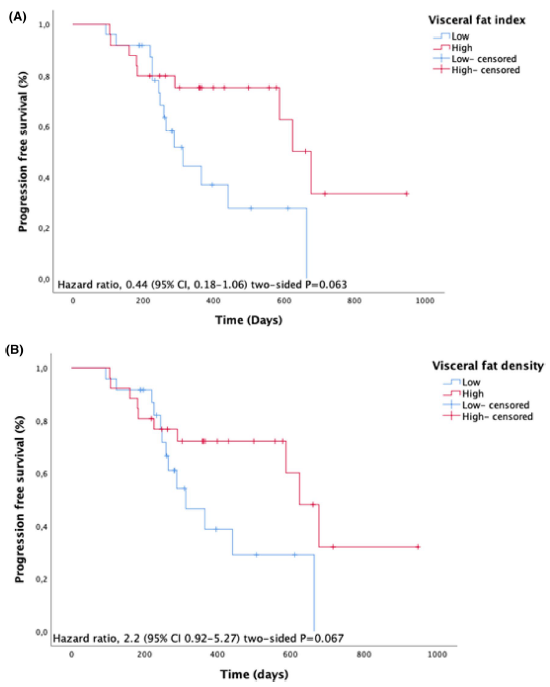
\includegraphics[scale=1.2]{Immagini/franzoi_VAT.png}
\caption{\label{fig:franzoi_VAT} \textit{Diagrammi di Kaplan-Meier della PFS divisi per indice di grasso viscerale alto e basso (A) e densità di grasso viscerale alta e bassa (B). Fonte:} \cite{Franzoi2020}.}
\end{figure}
\begin{figure}[htp]
\centering
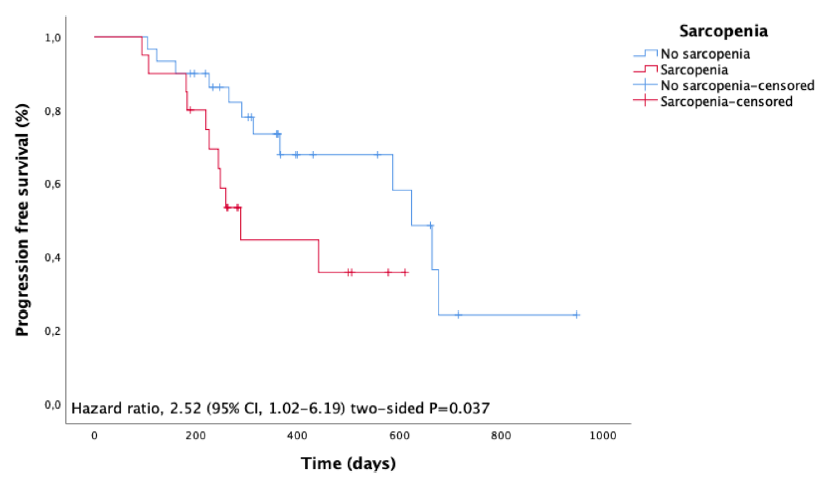
\includegraphics[scale=0.85]{Immagini/franzoi_sarcopenia.png}
\caption{\label{fig:franzoi_sarcopenia} \textit{Diagramma di Kaplan-Meier della PFS diviso in base alla presenza o meno di sarcopenia. Fonte:} \cite{Franzoi2020}.}
\end{figure}

È importante sottolineare che il suddetto effetto protettivo dell'obesità va inteso solo come una maggiore efficacia della terapia a inibitori nei pazienti sovrappeso e obesi rispetto ai pazienti sarcopenici, ma è interessante valutare cosa succede quando le due condizioni si presentano insieme in un paziente, come è stato fatto in un lavoro pionieristico di Prado \textit{et al.} \cite{Prado2008} già nel 2008. Lo scopo di questo lavoro era di accertare la prevalenza e le implicazioni cliniche, in pazienti affetti da carcinomi dei tratti respiratorio e gastrointestinale, dell'obesità sarcopenica, ritenuta a priori dagli autori come il peggior scenario possibile. Il peso e l’altezza dei pazienti sono stati registrati prima dell'inizio della terapia, i pazienti divisi in obesi e non obesi in base al loro BMI e classificati in base al loro stato funzionale, assegnato a ciascun paziente in accordo alle attività fisiche quotidiane riportate dai pazienti stessi. La massa muscolare è stata valutata mediante lo studio di \textit{slice} TC all'altezza della vertebra L3. La coorte iniziale includeva 2115 pazienti di cui il 15\% obesi, sebbene 6 mesi prima della prima misurazione la percentuale di obesi fosse del 27\%, in base alla storia delle variazioni di peso riportata dai pazienti stessi. Dei pazienti classificati come obesi solo 250 disponevano di TC adatte per l’analisi, di cui il 15\% è risultato avere sarcopenia mentre l’85\% no. Sono state trovate differenze significative nell'indice muscolare scheletrico e nella massa magra alipidica tra il campione di pazienti sarcopenici e il campione di pazienti non sarcopenici. L’attenuazione muscolare, misurata in HU, è risultata mediamente inferiore nei pazienti obesi affetti da sarcopenia, il che suggerisce infiltrazioni lipidiche nei muscoli per questa categoria di pazienti. Riguardo alla sopravvivenza, definita in questo caso come il numero di giorni di vita di ciascun paziente dopo la stima del BMI, sono state condotte analisi univariate e multivariate in base ai parametri principali (sesso, età, tipo di cancro, cambiamenti di peso, ecc.) e sono stati eseguiti \textit{log-rank test} per comparare le curve di sopravvivenza in base a ciascun parametro. Il dato più interessante è la comparazione delle curve di sopravvivenza tra pazienti obesi e obesi sarcopenici (\figref{fig:prado_obesitàsarcopenica}), che conferma l'importanza della sarcopenia come indicatore prognostico. Lo studio ha anche trovato indizi sul fatto che la prevalenza dell'obesità sarcopenica possa essere maggiore nei pazienti malati di cancro, sia perché l’obesità è un fattore di rischio per alcuni tipi di cancro, sia perché la sarcopenia è prevalente nei pazienti anziani, così come i tumori.
\begin{figure}[htp]
\centering
\includegraphics[scale=0.65]{Immagini/prado_obesitàsarcopenica.png}
\caption{\label{fig:prado_obesitàsarcopenica} \textit{Diagramma di Kaplan-Meier della sopravvivenza in pazienti obesi e obesi con presenza di sarcopenia. Fonte:} \cite{Prado2008}.}
\end{figure}

Ulteriore conferma all'inadeguatezza del BMI, ma anche della non totale affidabilità dei parametri calcolati mediante tomografia è data dallo studio di Magri \textit{et al.} \cite{Magri2019} sulla correlazione della stima della composizione corporea ottenuta tramite TC e di alcuni parametri metabolici con la sopravvivenza in pazienti affetti da cancro ai polmoni in cura con il nivolumab, un farmaco che stimola la risposta immunitaria contro le cellule tumorali. I parametri confrontati sono il BMI, l’indice di massa muscolare scheletrica (SMI), l’indice di massa magra alipidica (\textit{fat-free mass index}, FFMI), l’indice di massa grassa (FMI), i cambiamenti di peso e il livello di albumina nel sangue. Viene presa in considerazione l’albumina perché è una proteina il cui eccesso è associato a condizioni di malnutrizione o di forte dimagrimento (cachessia). Le misurazioni delle abbondanze dei diversi tessuti è stata effettuata su una singola \textit{slice} a livello della vertebra L3 acquisita con TC non prima di 10 settimane e non dopo 2 mesi rispetto all'inizio dell'immunoterapia. I livelli di albumina sono stati acquisiti non prima di 5 settimane e non dopo 2 settimane rispetto all'inizio dell'immunoterapia. Sorprendentemente, è stato trovato che solo i livelli di albumina e la perdita di peso erano correlati alla sopravvivenza dei pazienti, mentre le grandezze \textit{CT-derived} sono risultate parzialmente correlate con il BMI ma non con l’albumina e con la perdita di peso. Dall'analisi di Kaplan-Meier, gli autori del lavoro hanno trovato una minore sopravvivenza (intesa dall'inizio dell'immunoterapia) nei pazienti che presentavano una perdita di peso superiore al 5\% rispetto agli altri pazienti, e anche una minore sopravvivenza nei pazienti con livelli di albumina nel sangue più bassi del limite inferiore di normalità (\figref{fig:magri_sopravvivenza}). In questo studio, secondo gli autori il primo ad analizzare i cambiamenti di peso nei pazienti durante il primo approccio terapeutico, viene sottolineato per l’appunto il maggior valore prognostico e clinico di una semplice analisi del sangue per la misurazione dei livelli di albumina e del monitoraggio dei cambiamenti di peso rispetto alle grandezze \textit{CT-derived}.
\begin{figure}[htp]
\centering
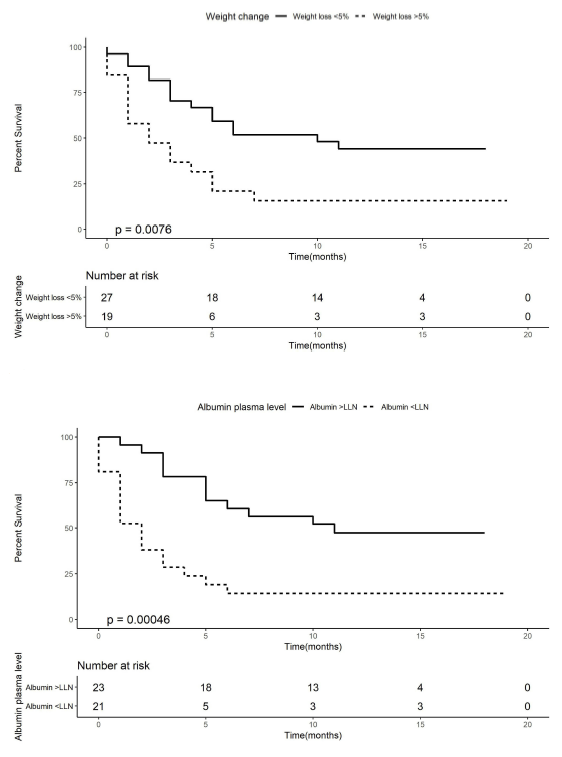
\includegraphics[scale=1.1]{Immagini/magri_sopravvivenza.png}
\caption{\label{fig:magri_sopravvivenza} \textit{Diagrammi di Kaplan-Meier della sopravvivenza divisi per perdita di peso, superiore o inferiore al 5\% (grafico in alto), e livello di albumina, inferiore o superiore rispetto al limite inferiore di normalità (grafico in basso). Fonte:} \cite{Magri2019}.}
\end{figure}

Il monitoraggio dei cambiamenti di peso è fondamentale per la buona riuscita di una terapia antitumorale, fondamentalmente perché la quantità di farmaco da somministrare al paziente si fonda sulla quantità di tessuto adiposo e muscolare. I cambiamenti di peso sono molto frequenti nei pazienti affetti da tumore: innanzitutto la diminuzione del peso senza cambi rilevanti nello stile di vita è uno dei primi campanelli d’allarme per la diagnosi stessa del tumore. In questa fase la diminuzione è causata da alterazioni metaboliche dovute alla risposta del sistema immunitario contro il tumore. Successivamente questo problema può aumentare a causa delle terapie antitumorali, sia la chemioterapia sia la radioterapia, che possono causare riduzione dell'appetito, debolezza muscolare, nausea, vomito e altri effetti collaterali \cite{aimac}. Accanto alla perdita di peso, in risposta ai trattamenti per alcuni tipi di tumori si può avere anche un aumento di peso, anche questo da non sottovalutare. Il caso più eclatante è l’aumento di peso dovuto alla chemioterapia adiuvante per pazienti colpiti da cancro alla mammella. Si tratta di una terapia che viene eseguita comunemente in seguito all'asportazione chirurgica del tumore per aumentare la probabilità di completa guarigione. È stato dimostrato che i pazienti che aumentano di peso più della media con questo tipo di trattamento hanno un maggior rischio di recidive e di morte \cite{Camoriano1990}. Ovviamente la soluzione migliore sarebbe impedire o minimizzare l’aumento di peso ma in ogni caso c’è bisogno di adeguare le cure sulla base della composizione corporea.
\clearpage
\null
\newpage
\chapter{Stima della \textit{body composition} con metodi automatici ed effetti del mezzo di contrasto}
Dopo aver esposto, nel capitolo \ref{capitolo2}, quali sono gli ambiti di interesse della segmentazione di alcuni tessuti corporei attraverso immagini TC, il presente lavoro di tesi ha come obiettivo quello di fare il punto sullo stato dell'arte della segmentazione automatica delle immagini TC per le strutture utili alla \textit{body composition}. Il presente capitolo, dunque, si articola in tre paragrafi: nel primo paragrafo viene svolto un discorso generale sulla segmentazione automatica di immagini TC mediante i risultati riportati in diversi articoli; il secondo tratta gli effetti che il mezzo di contrasto può avere sulle grandezze \textit{CT-derived}, e su come i software di segmentazione automatica e semiautomatica rispondono a questi effetti; infine, nel terzo ci si sofferma sui vantaggi dei metodi di segmentazione 3D.

\section{Stato dell'arte sulla segmentazione automatica dei tessuti corporei attraverso immagini TC}
Uno degli studi più recenti in questo ambito è quello svolto da Borrelli \textit{et al.} \cite{Borrelli2021}, in cui il software di segmentazione, basato su una rete neurale a convoluzione (CNN, di cui si tratta nel paragrafo \ref{retineurali}), è stato allenato su un \textit{training set} costituito da 50 scansioni TC ottenute da una coorte di 50 pazienti affetti da linfoma, con \textit{slice} dallo spessore di 3\,mm; il software è stato poi testato su \textit{test set} di 148 TC ottenute da un gruppo di 74 pazienti colpiti da tumore alla prostata, con \textit{slice} dallo spessore di 5\,mm. Entrambi i gruppi di scansioni sono stati acquisiti mediante un sistema integrato PET/TC. Le immagini TC del \textit{training set} sono state segmentate da uno specialista di medicina nucleare, limitatamente però al tessuto adiposo sottocutaneo (SAT) e al tessuto muscolare, escludendo quindi il tessuto adiposo viscerale (VAT). Sono stati così calcolati i volumi di SAT e muscolo dalla vertebra T11 fino alla zona caudale dell'osso iliaco; sono stati identificati come SAT i voxel (corrispettivo volumetrico del pixel) con HU compreso tra $-190$ e $-30$, come muscolo i voxel con HU compreso tra $-30$ e 150. Per il \textit{test set} è stata eseguita una segmentazione manuale su una sola \textit{slice} per acquisizione all'altezza della vertebra L3, usando gli stessi intervalli della scala Hounsfield di prima. Il software di segmentazione automatica utilizzato (sviluppato da RECOMIA, disponibile online e completamente gratuito \cite{recomia}) assegna a ogni pixel un valore da 0 a 1 e il singolo pixel viene poi assegnato alla categoria in cui ha ottenuto il punteggio più alto. Per valutare l’accuratezza della segmentazione effettuata dal software viene utilizzato il coefficiente di similarità di Dice, impiegato in questo specifico caso per calcolare la sovrapposizione tra le segmentazioni automatica e manuale in una singola \textit{slice} all'altezza della vertebra L3.
Dati due insiemi \textit{X} e \textit{Y}, il coefficiente di Dice è definito come:
\begin{equation}
    DC = \dfrac{2\,\abs{X \cap Y}}{\abs{X}+\abs{Y}}\,,
\end{equation}
dove $\abs{X}$ e $\abs{Y}$ sono le cardinalità dei due insiemi, cioè il numero di elementi di ciascun insieme \cite{dice}.

Tornando a quanto riportato in \cite{Borrelli2021}, il coefficiente di Dice medio per il \textit{test set} è risultato essere 0,96 per il SAT e 0,94 per il tessuto muscolare, indice di un ottimo accordo fra le segmentazioni manuale e automatica, di cui un esempio è presentato nella \figref{fig:borrelli_segmentazione}. Poiché il \textit{test set} era composto da due TC per ogni paziente, eseguite in media a tre giorni di distanza l’una dall'altra, è stata calcolata anche la riproducibilità della segmentazione automatica, che è risultata essere decisamente maggiore per i volumi piuttosto che per le singole \textit{slice}. La differenze relative fra i due studi sono risultate essere di 1,8\% e 5\% rispettivamente per i volumi e le superfici di SAT e di 1,9\% e 3,9\% rispettivamente per i volumi e le superfici di tessuto muscolare.
\begin{figure}[htp]
\centering
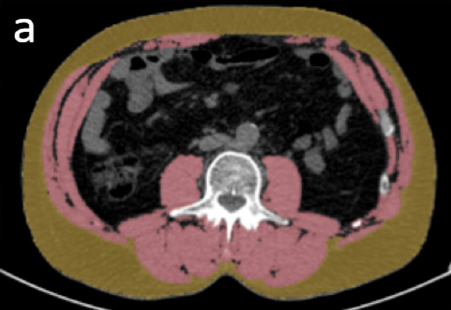
\includegraphics[scale=0.806]{Immagini/borrelli_manual.png}\quad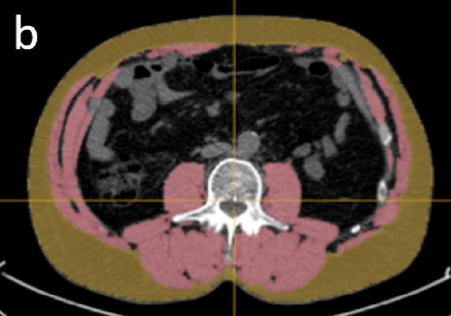
\includegraphics[scale=0.791]{Immagini/borrelli_ai.png}
\caption{\label{fig:borrelli_segmentazione} \textit{Segmentazione manuale (a) e automatica (b) di SAT (in marrone) e muscolo (in rosa) di una slice TC ad altezza L3. Fonte:} \cite{Borrelli2021}.}
\end{figure}

Un punto molto importante presente in \cite{Borrelli2021} è l'elaborazione di due modelli di regressione lineare, riportati nella \figref{fig:borrelli_regressione}, per predire i volumi dei tessuti a partire dalle superfici alla vertebra L3. Per il SAT, l’equazione della retta di regressione è $ y = 35,63\,x + 630,3 $, con un coefficiente di correlazione lineare $ r^2 = 0,83 $. Per il tessuto muscolare il modello è dato dall'equazione $ y = 40,15\,x + 1461 $, con $ r^2 = 0,64 $. Tutte le argomentazioni sopra riportate indicano una netta convenienza nell'utilizzare i volumi di SAT e muscolo piuttosto che le superfici a L3. Infine, nello studio viene messa in luce una limitazione del software di RECOMIA, in particolare dovuta al fatto che nel 9\% dei casi si sia reso necessario l’intervento di un radiologo per correggere la segmentazione proposta dal software stesso. Un’altra importante limitazione, assolutamente non banale, è il fatto che non sia stato preso in considerazione il VAT, assolutamente indispensabile nella formulazione, ad esempio, di un piano terapeutico.
\begin{figure}[htp]
\centering
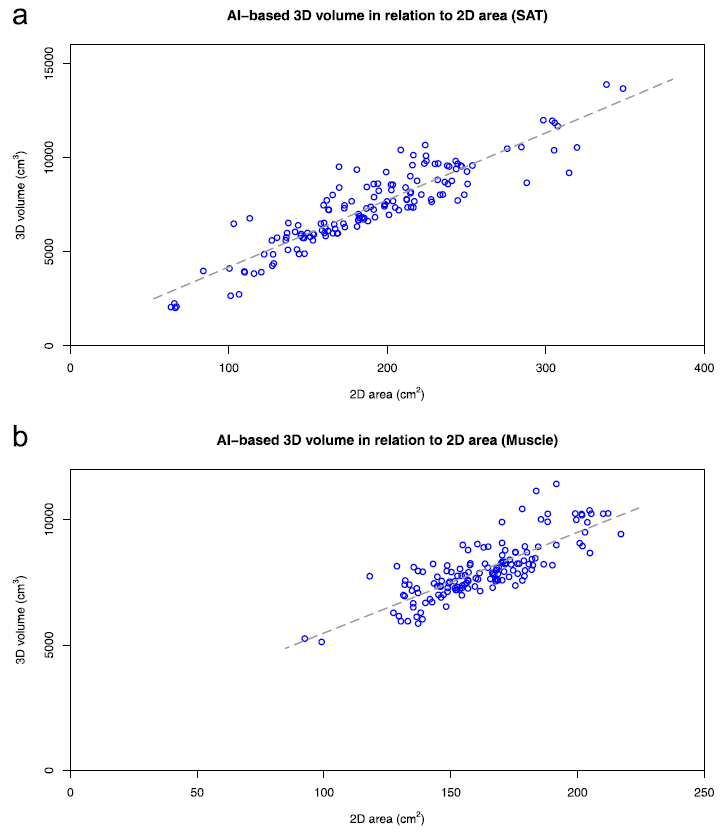
\includegraphics[scale=1]{Immagini/borrelli_regressione.png}
\caption{\label{fig:borrelli_regressione} \textit{Grafico di correlazione tra volumi e superfici di SAT (a) e muscolo (b) calcolati da segmentazione automatica di slice TC ad altezza L3. Fonte:} \cite{Borrelli2021}.}
\end{figure}

Uno studio su una coorte più ampia e differenziata è stato eseguito da Magudia \textit{et al.} \cite{Magudia2021}; anche questo lavoro ha lo scopo di dimostrare la validità della segmentazione automatica, effettuata con una U-Net, per il calcolo della composizione corporea, sempre mediante misurazioni effettuate a livello della vertebra L3, poiché queste sono ben correlate, solitamente, con SAT, VAT e muscolo scheletrico (SM) totali (in tutto il corpo). Il \textit{data set} di questo studio è costituito da 604 TC addominali, una per ogni paziente, tutti affetti da adenocarcinoma pancreatico: 421 TC sono state usate per l’allenamento, 94 per la validazione%
\footnote{Un \textit{data set} di validazione è un insieme di dati \virgolette{ibrido}, in quanto si tratta di un \textit{data set} considerato ancora di allenamento ma che viene utilizzato per testare l’apprendimento del software; tuttavia, non prende parte né nel processo di allenamento di basso livello né nella fase di \textit{testing} finale \cite{sets}.}
e 89 per il \textit{testing} del modello finale. I pazienti sono per il 49\% uomini e per il 51\% donne, con un’età media di 54 anni. È stato utilizzato anche un secondo, esterno \textit{test set} costituito da 534 TC addominali di pazienti colpiti da linfoma. Per la segmentazione manuale del \textit{training set} sono stati utilizzati gli stessi valori di HU dello studio precedente \cite[vedi][]{Borrelli2021}. La coorte su cui il software è stato impiegato è di 12128 membri, selezionati tra pazienti senza comorbidità oncologiche o cardiovascolari note, in modo da rendere lo studio rappresentativo della popolazione generale. Le associazioni tra le CSA dei diversi tessuti e parametri come età, sesso e razza sono state determinate con test di Student e regressioni lineari. Dall’SMI è stato trovato che il 35\% dei pazienti manifestava sarcopenia, diagnosticata per SMI inferiore a 55\,$\mathrm{cm}^2/\mathrm{m}^2$ per gli uomini e 39\,$\mathrm{cm}^2/\mathrm{m}^2$ per le donne. I coefficienti di Dice per SM, SAT e VAT sono stati calcolati rispettivamente in $0,97\pm0,03$, $0,98\pm0,02$ e $0,95\pm0,10$; l'accuratezza delle segmentazione automatica è constatabile, oltre che dai coefficienti di Dice, anche dall'esempio riportato nella \figref{fig:magudia_segmentazione}.
\begin{figure}[t]
\centering
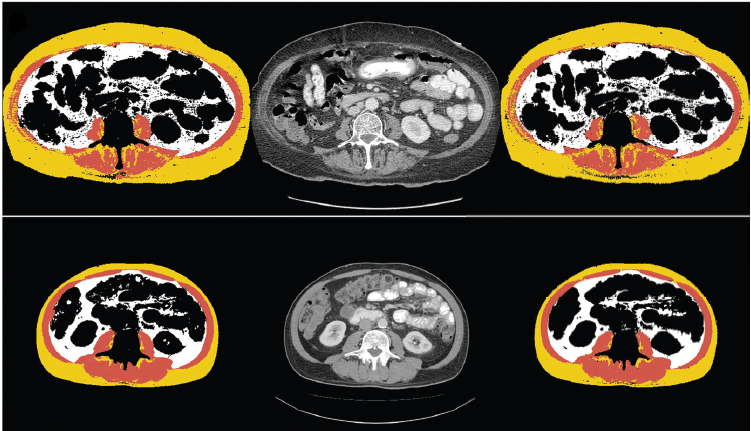
\includegraphics[scale=0.99]{Immagini/magudia_segmentazione.png}
\caption{\label{fig:magudia_segmentazione} \textit{Slice TC ad altezza L3 (al centro) e loro segmentazioni automatiche (a sinistra) e manuali (a destra). Il muscolo scheletrico è evidenziato in marrone, il grasso sottocutaneo in giallo e il grasso viscerale in bianco, mentre tutto il resto è riportato in nero. Fonte:} \cite{Magudia2021}.}
\end{figure}
Sono state calcolate curve di riferimento sia per le CSA di ciascuna tipologia di tessuto sia per i loro indici (vale a dire le superfici di ciascun tessuto divise per l’altezza al quadrato di ciascun paziente) in funzione di età, sesso e razza. Come ci si aspettava, sono state trovate CSA maggiori di SM e VAT e CSA lievemente minori di SAT negli uomini rispetto alle donne. Altri risultati sono l’aumento generale di VAT con l’aumentare dell'età e allo stesso tempo la perdita di SM, come riportato nei grafici di \figref{fig:magudia_smvat}. La CSA di SM è più o meno simile confrontando pazienti bianchi e pazienti neri, mentre i pazienti neri dimostrano valori di VAT generalmente più bassi dei bianchi. In ogni caso, il fatto più interessante è proprio che le curve di riferimento attestino differenze fra i gruppi etnici nella composizione corporea, cosa che invece non si riesce a dimostrare utilizzando il peso o l’indice di massa corporea.
\begin{figure}[htp]
\centering
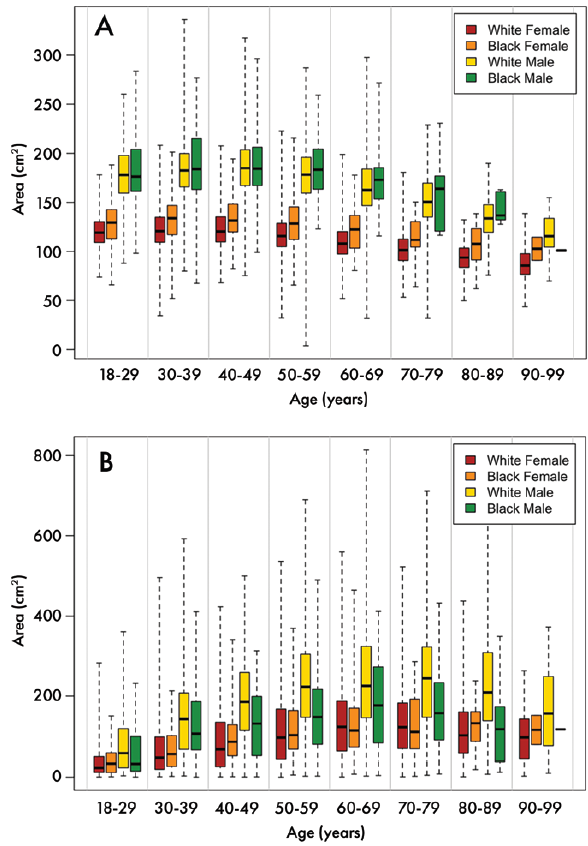
\includegraphics[scale=0.95]{Immagini/magudia_smvat.png}
\caption{\label{fig:magudia_smvat} \textit{Grafici delle CSA di muscolo scheletrico (A) e grasso viscerale (B), con popolazione divisa per sesso e razza. Fonte:} \cite{Magudia2021}.}
\end{figure}

In \cite{Hemke2020} viene testata una rete neurale a convoluzione per la segmentazione automatica dei tessuti corporei, non come al solito all'altezza di L3 ma nella regione pelvica. Il \textit{data set} è costituito da TC addominali di 200 pazienti, di cui 180 sono state utilizzate per l’allenamento e 20 per testare la CNN. Questo lavoro si distingue dagli altri perché tiene in considerazione ben 6 regioni diverse: oltre ai pixel di sfondo, vengono classificati SAT, muscolo, tessuto adiposo intermuscolare (IMAT), osso e tutto il rimanente contenuto intrapelvico (viscere e VAT). I risultati ottenuti nel calcolo della massa muscolare sono comparabili con quelli di altri lavori eseguiti con metodi automatici all'altezza delle vertebre L3 e L4. L’importanza dello studio della regione pelvica sta nell'associazione di alcuni disordini neuromuscolari con infiltrazioni adipose e atrofia della regione pelvica. Sebbene il volume muscolare \textit{total body} sia fortemente correlato con \textit{slice} trasversali della regione L3-L4, misure del grado di sarcopenia a quell'altezza possono essere anche molto diverse da misure effettuate su altre vertebre. Questo elemento può generare valutazioni errate se viene presa in considerazione solamente la regione L3-L4: ad esempio, la massa muscolare della regione pelvica, funzionalmente molto importante per la motilità degli arti inferiori, è di solito maggiore rispetto alla massa muscolare di L3-L4. I coefficienti di Dice per le varie regioni sono riportati in \tabref{tab:dice}; i valori trovati sono comparabili con quelli ottenuti all'altezza di L3 negli altri studi presentati precedentemente. Un esempio dell'accuratezza della CNN impiegata è riportato nella \figref{fig:hemke_segmentazione}; d'altra parte il software ha mostrato difficoltà nel distinguere regioni di confine, come quelle tra muscoli e viscere (\figref{fig:hemke_viscere}) e lungo la fascia muscolare addominale (\figref{fig:hemke_fascia}).
\begin{table}[htp]
    \centering
    \begin{tabular}{|c|c|}
        \hline
        \textit{Label}                      & Coefficiente di Dice  \\ \hline
        Sfondo                              & 1                     \\
        Tessuto adiposo sottocutaneo        & 0,97                  \\
        Tessuto muscolare                   & 0,95                  \\
        Tessuto adiposo intermuscolare      & 0,91                  \\
        Tessuto osseo                       & 0,92                  \\
        Tessuto adiposo viscerale e viscere & 0,98                  \\ \hline
    \end{tabular}
    \caption{\textit{Coefficienti di Dice per tessuto da immagini TC della regione pelvica}.}
    \label{tab:dice}
\end{table}

\begin{figure}[htp]
\centering
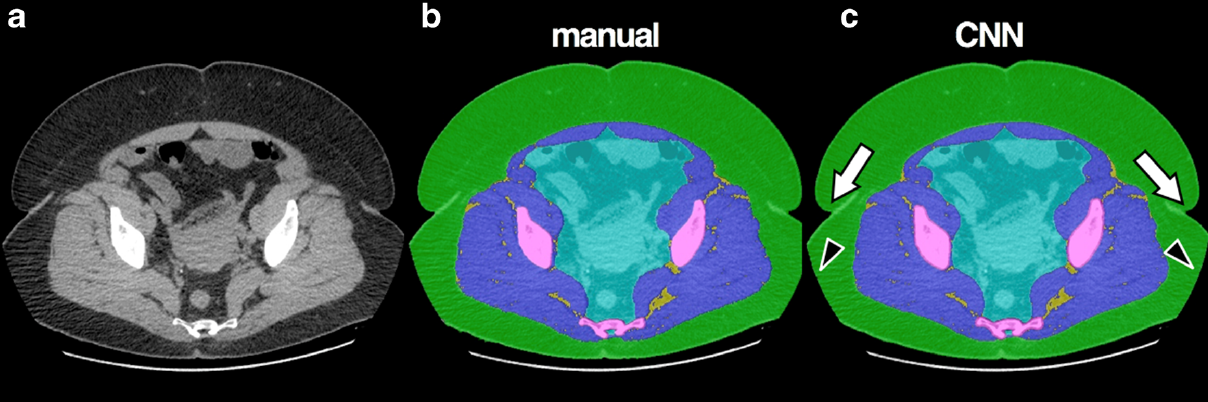
\includegraphics[scale=0.615]{Immagini/hemke_segmentazione.png}
\caption{\label{fig:hemke_segmentazione} \textit{Immagine TC (a) e sue segmentazioni manuale (b) e automatica (c), caratterizzata da una quantità elevata di SAT. Ai tessuti sono assegnati seguenti colori: verde per il SAT, giallo per l'IMAT, magenta per l'osso, blu per il muscolo e azzurro per le viscere e il VAT. La CNN ha dimostrato un buon comportamento anche in situazioni non scontate, come nel riconoscere le pieghe della pelle (freccia bianca) e il cut-off del campo visivo della scansione (freccia nera). Fonte:} \cite{Hemke2020}.}
\end{figure}
\begin{figure}[htp]
\centering
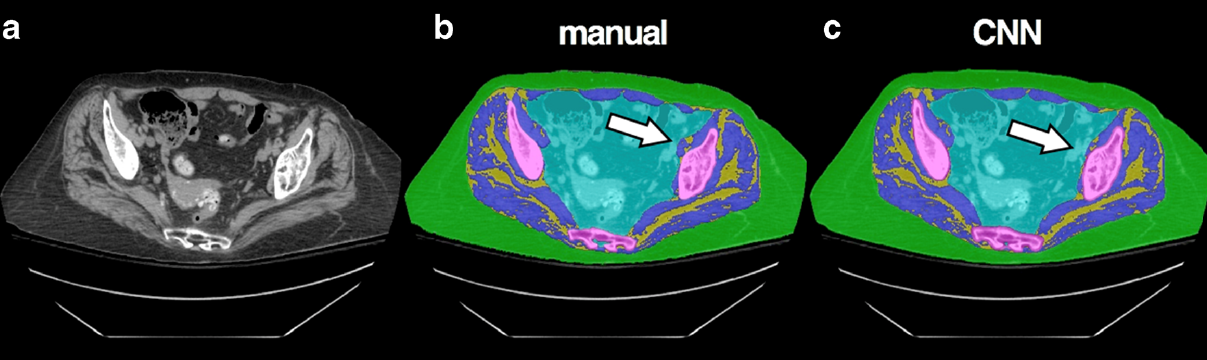
\includegraphics[scale=0.615]{Immagini/hemke_viscere.png}
\caption{\label{fig:hemke_viscere} \textit{Immagine TC (a) e sue segmentazioni manuale (b) e automatica (c), caratterizzata da una quantità elevata di IMAT. La freccia bianca indica una piccola porzione di tessuto che la CNN riconosce come viscere, mentre in realtà si tratta di muscolo. Fonte:} \cite{Hemke2020}.}
\end{figure}
\begin{figure}[htp]
\centering
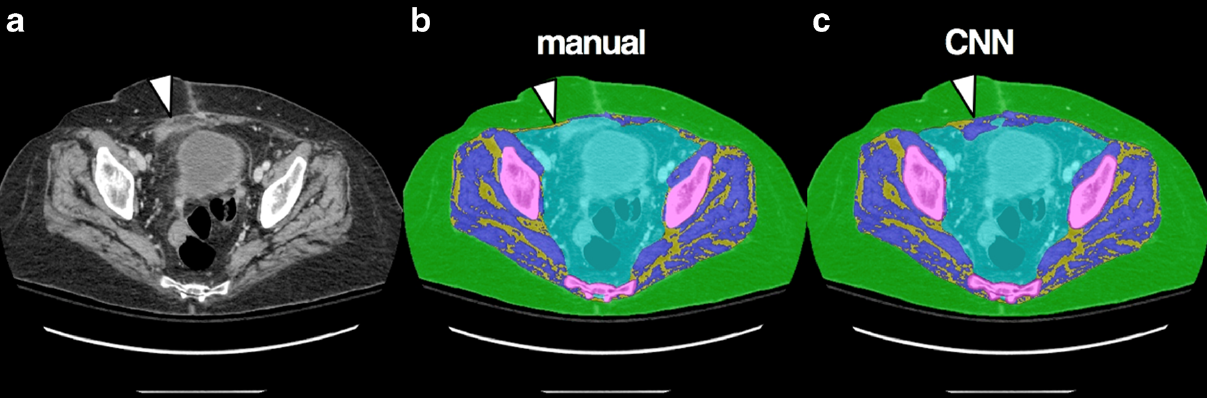
\includegraphics[scale=0.615]{Immagini/hemke_fascia.png}
\caption{\label{fig:hemke_fascia} \textit{Immagine TC (a) e sue segmentazioni manuale (b) e automatica (c). La freccia bianca indica una piccola porzione di tessuto che la CNN riconosce come muscolo, mentre in realtà si tratta di tessuto viscerale misto e grasso viscerale. Fonte:} \cite{Hemke2020}.}
\end{figure}

\section{Effetti del mezzo di contrasto sulle grandezze \textit{CT-derived}}
I mezzi di contrasto sono sostanze che vengono somministrate ai pazienti prima o durante un qualche esame diagnostico (TC, \textit{imaging} di risonanza magnetica, esami con ultrasuoni) per permettere al radiologo di evidenziare condizioni patologiche all'interno di un’immagine e, in generale, di migliorare la qualità dell'immagine, aumentando il contrasto fra una regione del corpo e le regioni circostanti. Un mezzo di contrasto può essere somministrato per via orale, rettale o intravenosa. Per la TC e le immagini radiologiche in generale, il mezzo di contrasto può essere una soluzione a base di iodio, immessa nel corpo per via endovenosa o in cavità varie, oppure un composto a base di solfato di bario, somministrato in questo caso per via orale in diverse forme \cite{contrast}. L’effetto del mezzo di contrasto si esprime in un cambio del coefficiente di attenuazione lineare dei tessuti, quindi in un cambio di valori all'interno della scala Hounsfield. Questo rappresenta un problema per un algoritmo di segmentazione, che viene calibrato in base a certi valori di HU per ciascun tipo di tessuto, e che di conseguenza potrebbe fallire nel caso in cui le immagini da analizzare siano influenzate dal mezzo di contrasto. Diventa importante, di conseguenza, indagare come cambiano i valori di HU quando al paziente viene somministrato un mezzo di contrasto.

Per cominciare, uno studio di Fuchs \textit{et al.} \cite{Fuchs2018} ha investigato l’effetto del mezzo di contrasto intravenoso (IV) sulle misure di superficie (\textit{cross sectional skeletal muscle area}, CSMA) e densità (\textit{skeletal muscle density}, SMD) del tessuto muscolare scheletrico, all'interno di un esame angiografico eseguito mediante TC (\textit{computed tomography angiography}, CTA). Le misure di CSMA e SMD sono state eseguite a livello della vertebra L3, su un \textit{data set} costituito da 114 immagini estratte da 38 CTA. La soglia di definizione del muscolo scheletrico è stata definita, come al solito, tra $-29$ e 150\,HU, mentre la SMD è stata definita come l’attenuazione media della superficie di muscolo segmentata. I valori di CSMA e SMD sono stati registrati su ciascun paziente durante la stessa indagine diagnostica e confrontati con altre serie di valori acquisiti durante la stessa indagine variando specifici parametri tecnici; il confronto fra le serie di dati è stato effettuato mediante il metodo Bland-Altman, presentato nel paragrafo \ref{blandaltman}. La segmentazione è stata effettuata con un software semiautomatico. Confrontando le superfici misurate su \textit{slice} spesse 2\,mm con e senza mezzo di contrasto, sono stati rilevati valori di CSMA significativamente più alti nel primo caso rispetto al secondo: in una media su tutti i pazienti, la superficie trasversale è risultata maggiore dell'1,88\%; lo stesso vale per l’SMD, più grande del 5,99\% nelle immagini con mezzo di contrasto rispetto a quelle senza.

Nello stesso studio, su un altro \textit{data set} costituito da 102 immagini estratte da 38 PET/TC (senza mezzo di contrasto), sono state svolte analisi sulle dipendenze di CSMA e SMD dallo spessore delle \textit{slice} e dalla corrente del tubo a raggi X. Tralasciando il secondo punto, che richiederebbe una discussione che esula dallo scopo di questa tesi, sono stati trovati dati interessanti riguardo allo spessore delle \textit{slice}: è stato rilevato un aumento medio dell'1,11\% della CSMA all'altezza di L3 se si impiega una \textit{slice} dello spessore di 5\,mm rispetto a una dello spessore di 2\,mm; parallelamente, i valori di SMD sono minori dell'11,64\% per i 5\,mm rispetto ai 2\,mm. Nella \figref{fig:fuchs_ba} sono riportati i grafici di Bland-Altman riguardanti le dipendenze di CSMA e SMD appena esposte.
\begin{figure}[H]
\centering
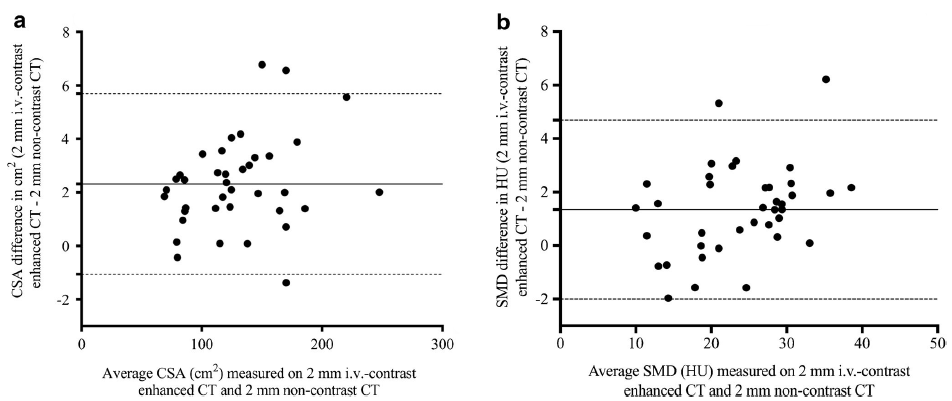
\includegraphics[scale=0.78]{Immagini/fuchs_contrasto.png}\quad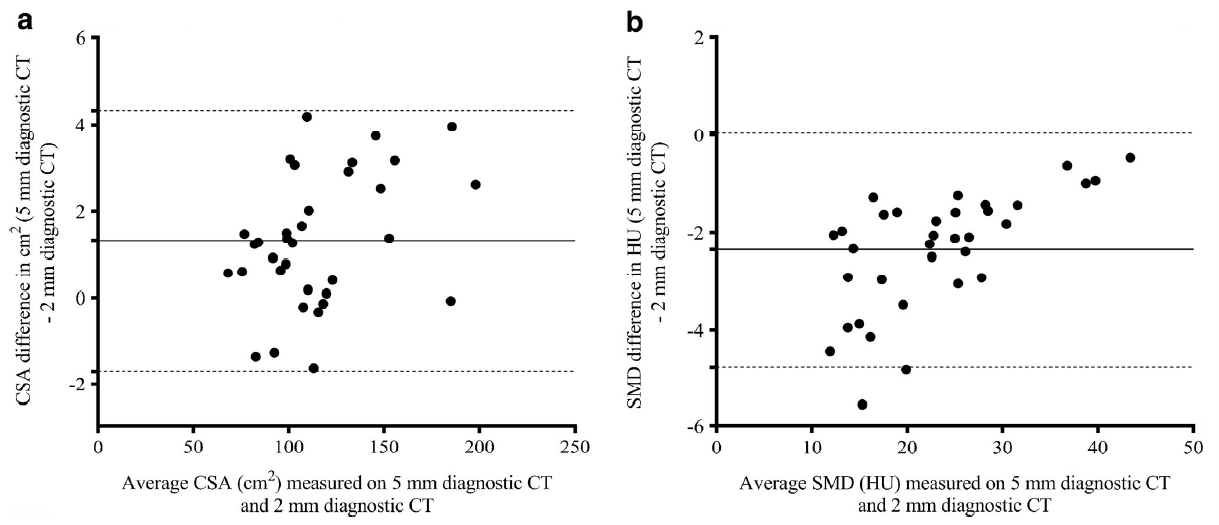
\includegraphics[scale=0.61]{Immagini/fuchs_spessore.png}
\caption{\label{fig:fuchs_ba} \textit{Grafici di Bland-Altman di cross-sectional muscle area (CSMA) (a) e densità di muscolo scheletrico (SMD) (b): in alto, differenze misurate su slice di $2\,\textnormal{mm}$ da acquisizioni con e senza mezzo di contrasto; in basso, differenze misurate su slice di $5\,\textnormal{mm}$ e di $2\,\textnormal{mm}$. I grafici sono riportati in funzione del valore medio della grandezza corrispondente. La linea continua rappresenta la differenza media, mentre le linee tratteggiate rappresentano i limiti di concordanza. Fonte:} \cite{Fuchs2018}.}
\end{figure}

I motivi dei due fenomeni descritti sono facili da intuire: innanzitutto, il mezzo di contrasto è più denso dei tessuti corporei, quindi aumenta i valori di HU dei tessuti che normalmente si troverebbero sotto il \textit{threshold}. \textit{Slice} più sottili, invece, forniscono misure più accurate a causa del minor volume analizzato; allo stesso tempo, più una \textit{slice} è sottile più è soggetta a rumore, comparata con una più spessa. Nella \figref{fig:fuchs_2} sono riportati gli istogrammi del numero di pixel in funzione delle unità Hounsfield, che presentano in maniera particolarmente intuitiva i fenomeni appena descritti. Poiché l’utilizzo del mezzo di contrasto IV e lo spessore delle \textit{slice} influenzano in maniera significativa i risultati, influenzeranno di conseguenza eventuali diagnosi di sarcopenia, che saranno a loro volta associate a un certo rischio di morte: ciò rende indispensabile la considerazione di questi parametri sia in lavori scientifici, dove capita ad esempio che lo spessore delle \textit{slice} non sia riportato, sia per la formulazione di diagnosi, quindi in fase di progettazione di un algoritmo per la segmentazione automatica.
\begin{figure}[htp]
\centering
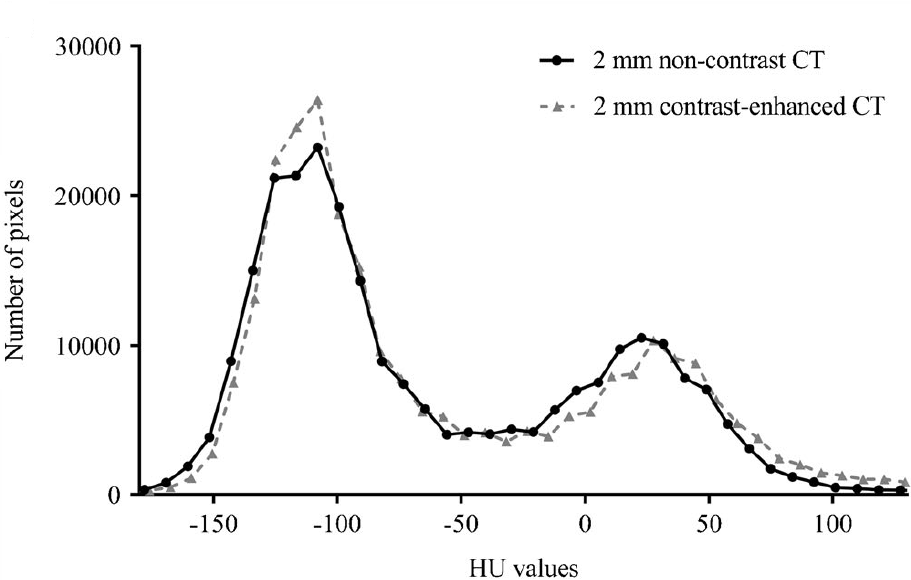
\includegraphics[scale=0.65]{Immagini/fuchs_contrasto2.png}\quad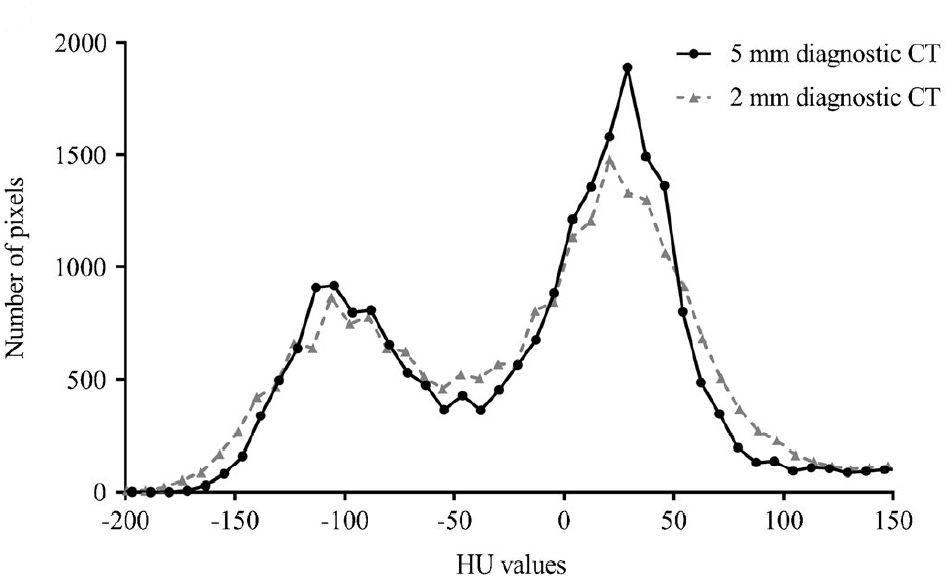
\includegraphics[scale=0.65]{Immagini/fuchs_spessore2.png}
\caption{\label{fig:fuchs_2} \textit{Istogrammi delle immagini TC che mostrano il numero di pixel in funzione delle unità Hounsfield per acquisizioni di slice di $2\,\mathrm{mm}$ con e senza contrasto (immagine di sinistra) e per acquisizioni senza contrasto di slice di $2$ e $5\,\mathrm{mm}$. Si può notare: nell'immagine di sinistra, un numero maggiore di pixel nell'intervallo compreso tra $-120$ e $-100\,\mathrm{HU}$ (tessuto adiposo) per le acquisizioni contrast-enhanced rispetto alle acquisizioni unenhanced; nell'immagine di destra, un numero maggiore di pixel nell'intervallo compreso tra $0$ e $50\,\mathrm{HU}$ (tessuto adiposo e muscolare) per le acquisizioni di slice di $5\,\mathrm{mm}$ rispetto a quelle di $2\,\mathrm{mm}$. Fonte:} \cite{Fuchs2018}.}
\end{figure}

Un altro studio in cui vengono comparate la massa e la densità di muscolo scheletrico nelle differenti fasi di azione del mezzo di contrasto è quello svolto da van Vugt \textit{et al.} \cite{vanVugt2018}. Il \textit{data set} è costituito da TC di 50 pazienti con cancro o in attesa di trapianto di fegato, classificati in quattro categorie mediante il BMI (sottopeso, normopeso, sovrappeso e obesi). Per l’acquisizione di tutte le TC è stato seguito un protocollo standard pianificato in modo da poter distinguere tre fasi durante lo svolgimento delle indagini diagnostiche. Le fasi sono le seguenti: fase \textit{unenhanced} (mezzo di contrasto non ancora somministrato), fase arteriosa e fase venosa portale. Innanzitutto, si esegue una TC senza contrasto, poi viene iniettato il mezzo di contrasto IV, in quantità variabile in base al peso del paziente (minore o maggiore di 80\,kg). 30-35\,s dopo l’iniezione del contrasto IV inizia la fase arteriosa, che consente di vedere lesioni ipervascolarizzate da rami dell'arteria epatica; alla fase arteriosa subentra la fase venosa portale, circa 70\,s dopo l’infusione del contrasto, in cui è possibile valutare quali lesioni sono vascolarizzate dai rami della vena porta \cite{passariello}, un sistema vascolare che ha il compito di convogliare al fegato il sangue proveniente dal tratto gastrointestinale, dal pancreas e dalla milza \cite{porta}. L’inizio della fase arteriosa è stato determinato ponendo una regione d’interesse nell'aorta addominale superiore: l’inizio dell'acquisizione è stato impostato per avvenire 15\,s dopo il raggiungimento di 100\,HU in quella zona. Lo spessore delle \textit{slice} è di 3\,mm in tutte le fasi. La CSMA è stata misurata all'altezza della vertebra L3 in tutte le fasi mediante un software di segmentazione semiautomatica, con il solito intervallo nella scala Hounsfield tra $-30$ e 150\,HU. Dividendo la CSMA espressa in centimetri quadrati per l’altezza del paziente al quadrato espressa in metri quadrati, è stato calcolato l’indice di muscolo scheletrico (SMI). La coorte di pazienti era composta per il 46\% da uomini e per il 54\% da donne; inoltre, il 38\% dei pazienti era sovrappeso e l’8\% obeso. Al variare delle fasi è stato osservato un cambiamento nell’SMI, che è risultato essere $(42,5 \pm 9,9)\,\text{cm}^2/\text{m}^2$ nella fase \textit{unenhanced} (prima della somministrazione del contrasto IV), $(42,8 \pm 9,9)\,\text{cm}^2/\text{m}^2$ nella fase arteriosa e $(43,6 \pm 9,9)\,\text{cm}^2/\text{m}^2$ nella fase venosa portale. Una variazione significativa è stata rilevata anche nella SMD, corrispondente a $(30,9 \pm 8,0)$\,HU nella fase \textit{unenhanced}, a $(38,0 \pm 9,9)$\,HU nella fase arteriosa e a $(38,7 \pm 9,2)$\,HU nella fase venosa portale. I dati sulle variazioni di SMI e SMD sono riportati nella \figref{fig:vanVugt_sm}, mentre le differenze tra le diverse fasi sono espresse in forma di grafici di Bland-Altman nelle figure \ref{fig:vanVugt_smiba} e \ref{fig:vanVugt_smdba}. In base alle misure effettuate, secondo le soglie definite in letteratura, è risultato avere bassa SMD durante la fase \textit{unenhanced} l’80\% dei pazienti, durante la fase arteriosa il 50\% e durante la fase venosa portale il 38\%.
\begin{figure}[htp]
\centering
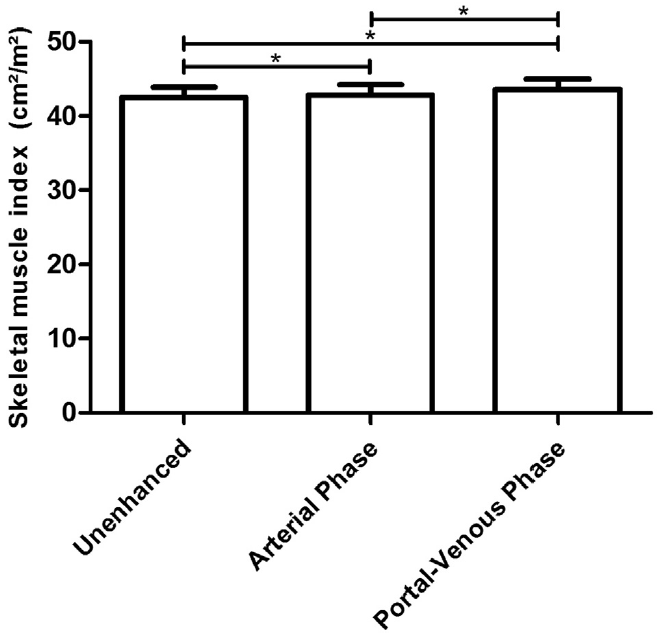
\includegraphics[scale=0.55]{Immagini/vanVugt_smi.png}\quad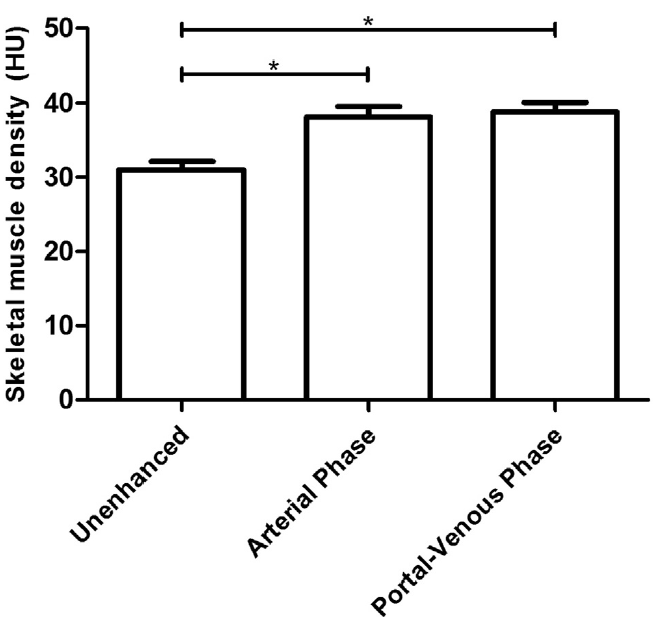
\includegraphics[scale=0.55]{Immagini/vanVugt_smd.png} \vspace{-25pt}
\caption{\label{fig:vanVugt_sm} \textit{Istogrammi di indice di muscolo scheletrico medio (immagine di sinistra) e densità di muscolo scheletrico media (immagine di destra) per fase di contrasto. Le barre di errore rappresentano la deviazione standard della media. Gli asterischi indicano differenze statisticamente significative tra i valori calcolati nelle varie fasi. Fonte:} \cite{vanVugt2018}.}
\end{figure}

\vspace{-5pt}Dalla comparazione delle CSMA è risultata, nella fase \textit{unenhanced}, una percentuale di pazienti sarcopenici sul totale del 44\%, che scende al 42\% nella fase arteriosa e risale al 48\% nella fase venosa portale. La quantità di mezzo di contrasto iniettato in ciascun paziente in base alla sua massa corporea non ha dimostrato nessuna correlazione con la SMD. Sebbene la dipendenza della massa muscolare scheletrica dalla fase sia stata trovata e sia statisticamente significativa, clinicamente il dato importante è quello sulla densità muscolare scheletrica, in quanto maggiormente legato alla diagnosi e alla valutazione del grado di sarcopenia e anche perché correlato al grado di infiltrazioni lipidiche all'interno dei muscoli scheletrici. Nonostante ciò, una massa muscolare scheletrica ridotta è associata a una maggiore tossicità delle terapie antitumorali, dunque è anch'essa importante in fase di definizione e aggiornamento dei piani terapeutici chemioterapici. Gli autori dello studio concludono sottolineando i vantaggi, per una maggiore coerenza e comparabilità tra lavori diversi, di utilizzare preferibilmente TC in fase venosa portale, poiché questo è il tipo di indagine eseguito più spesso per i pazienti malati di cancro; un altro consiglio è di riportare quantomeno la fase in cui vengono acquisite le TC utilizzate.

\begin{figure}[htp]
\centering
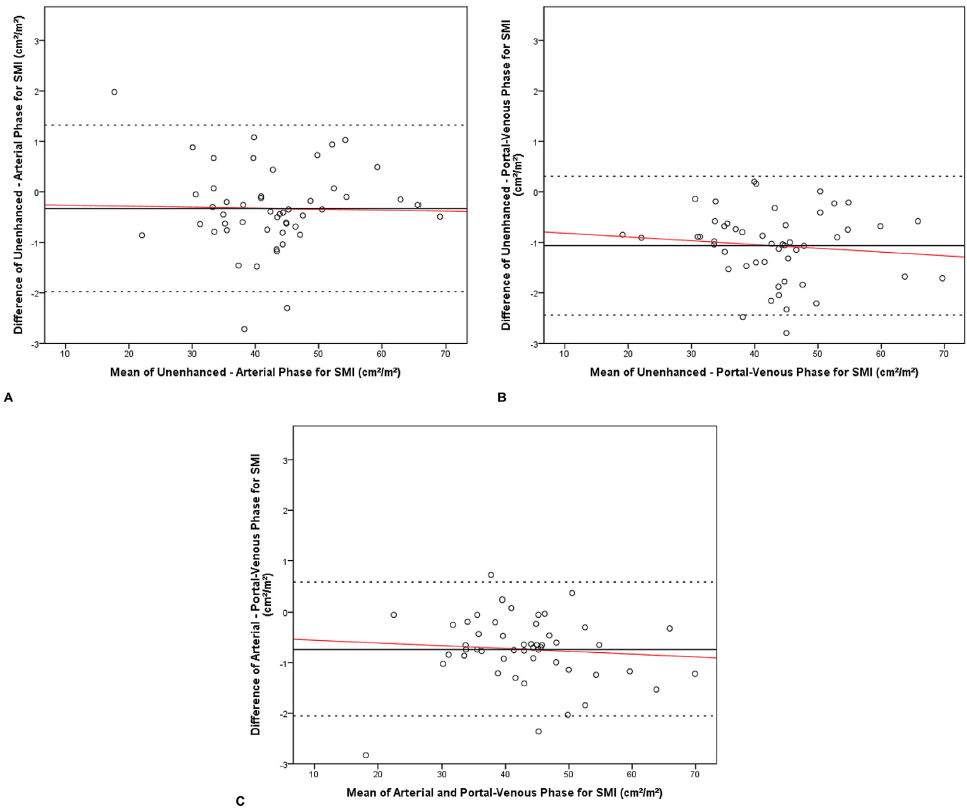
\includegraphics[scale=0.77]{Immagini/vanVugt_smiba.png}
\caption{\label{fig:vanVugt_smiba} \textit{Grafici di Bland-Altman dell'indice di muscolo scheletrico (SMI) per il confronto di: fase unenhanced e fase arteriosa (A), fase unenhanced e fase venosa portale (B) e fase arteriosa e fase venosa portale (C). La linea nera continua rappresenta la differenza media, le linee tratteggiate costituiscono i limiti di concordanza e la linea rossa è la retta di regressione. Fonte:} \cite{vanVugt2018}.}
\end{figure}
\begin{figure}[htp]
\centering
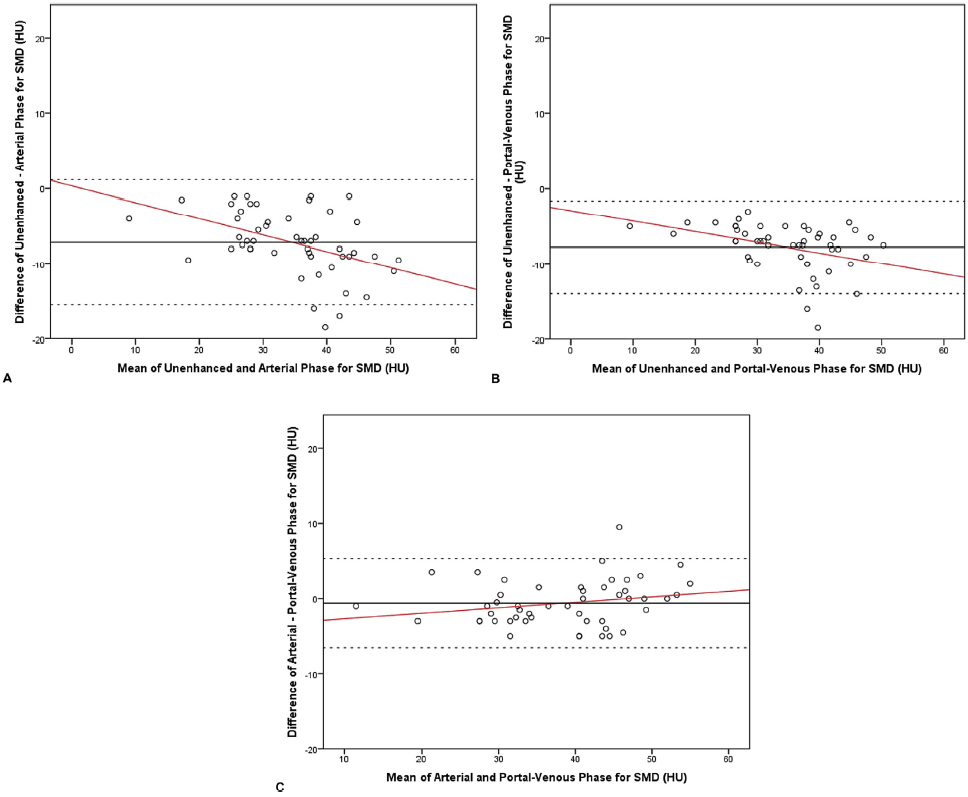
\includegraphics[scale=0.77]{Immagini/vanVugt_smdba.png}
\caption{\label{fig:vanVugt_smdba} \textit{Grafici di Bland-Altman della densità di muscolo scheletrico (SMD) per il confronto di: fase unenhanced e fase arteriosa (A), fase unenhanced e fase venosa portale (B) e fase arteriosa e fase venosa portale (C). La linea nera continua rappresenta la differenza media, le linee tratteggiate costituiscono i limiti di concordanza e la linea rossa è la retta di regressione. Fonte:} \cite{vanVugt2018}.}
\end{figure}

Nei due studi precedenti trova conferma la sospetta necessità di tenere in considerazione il mezzo di contrasto durante lo sviluppo di un software per la segmentazione automatica, a causa delle differenze sostanziali fra i dati ottenuti senza mezzo di contrasto e quelli ottenuti con contrasto IV nelle diverse fasi. Sulla base dei risultati trovati per il tessuto muscolare, ci si potrebbe aspettare risultati analoghi anche per il tessuto adiposo, importante quanto il primo nell'ambito della segmentazione e dei risvolti clinici.
Uno studio analogo a \cite{Fuchs2018}, ma che analizza oltre all'effetto dello spessore delle \textit{slice} e del mezzo di contrasto sui muscoli, anche quello sul tessuto adiposo, è stato realizzato da Morsbach \textit{et al.} \cite{Morsbach2019} su una coorte di 20 pazienti (13 uomini e 7 donne) di età compresa fra 40 e 87 anni, BMI medio di 21,2\,kg/$\text{cm}^2$, con sospetto carcinoma epatocellulare. Il \textit{data set} è costituito da una TC perfusionale per ciascun paziente, con almeno 4 serie acquisite senza mezzo di contrasto e inclusive di una scansione dell'addome ad altezza L3. In una TC di perfusione vengono eseguite delle scansioni a intervalli di 1,5-3\,s che danno luogo a delle serie mirate allo studio del flusso del mezzo di contrasto nei vasi sanguigni, in modo da fornire informazioni sulla vascolarizzazione di un eventuale  tumore. La scansione inizia qualche secondo prima che il mezzo di contrasto si sia diffuso per acquisire anche serie senza mezzo di contrasto. Per la valutazione dell'effetto del mezzo di contrasto sono state ricostruite 18 immagini a livello di L3 da 18 serie, di cui 4 in fase \textit{unenhanced}, 12 in fase arteriosa e 2 in fase venosa portale iniziale; le immagini sono state ricostruite a partire da \textit{slice} dello spessore di 5\,mm. Per valutare l’effetto dello spessore delle \textit{slice} sono state considerate immagini ad altezza L3 da \textit{slice} dello spessore di 2, 3, 4, 5 e 10\,mm, ricostruite dalle 4 serie acquisite durante la fase \textit{unenhanced}. Le immagini sono state segmentate manualmente da un radiologo, sono state calcolate CSA e attenuazione media (da cui si ricava la densità) di ogni tipo di tessuto e anche SMI, indice di tessuto adiposo e superficie di muscolo steatosico (muscolo infiltrato da tessuto adiposo).

Per quanto riguarda la dipendenza dal mezzo di contrasto, è stato rilevato un incremento di SMI con il progredire delle fasi del contrasto (2,8\% di variazione tra l’ultima serie e la prima) e una diminuzione di superficie di muscolo steatosico ($-13,8\%$) e dell'indice di tessuto adiposo ($-6,5\%$). Altri due parametri da segnalare sono l’attenuazione muscolare media, che presenta un incremento del 20\%, passando da 30\,HU nella fase \textit{unenhanced} a 36\,HU nella fase venosa portale, e l’attenuazione adiposa media, con un incremento di circa il 3,3\%, da $-90$\,HU a $-87$\,HU. Riguardo all'effetto dello spessore delle \textit{slice} sono stati trovati incrementi medi dell’1,9\% per l’SMI, del 3,3\% per la superficie muscolare steatosica e dell’1,5\% per l’indice di tessuto adiposo. Nessuna dipendenza è stata trovata in relazione all'attuazione muscolare, mentre per l’attenuazione adiposa è stato rilevato un incremento del 5,5\%.

Nel significativo aumento dell'attenuazione muscolare in relazione alle fasi del contrasto, trovano conferma gli errori metodologici evidenziati negli studi precedenti, che portano a una sovrastima della CSMA e della stessa attenuazione muscolare; gli autori sottolineano la necessità di un protocollo standardizzato per la valutazione della composizione corporea mediante TC. Similmente a quanto riportato dal gruppo di lavoro di Fuchs in \cite{Fuchs2018}, anche in questo studio si trovano delle dipendenze significative di tutti i parametri dallo spessore delle \textit{slice} tranne, sorprendentemente, per quanto riguarda l’attenuazione muscolare.

Un lavoro più specifico sulla dipendenza della segmentazione del tessuto adiposo dai parametri di acquisizione è quello presentato da Troschel \textit{et al.} \cite{Troschel2021}, che ha l'obiettivo di stimare l’influenza del contrasto IV e dello spessore delle \textit{slice} su CSA e attenuazione media di tessuto adiposo sottocutaneo (SAT), viscerale (VAT) e intermuscolare (IMAT). Il \textit{data set} consiste di immagini ottenute con tre tipi di tecniche: \textit{computed tomography angiography} (CTA), \textit{dual-energy CT} (DECT)%
\footnote{La DECT è una tecnica che utilizza due fasci di raggi X di diversa energia, in modo da poter identificare meglio sostanze diverse. Ciò è reso possibile dal fatto che ciascun elemento chimico è caratterizzato da una propria energia di legame della \textit{shell} K, cioè la \textit{shell} più interna di un atomo; c’è più probabilità che un fotone X venga assorbito, generando effetto fotoelettrico, se questo ha energia simile all'energia di legame della \textit{shell} K. L’aumento della probabilità di assorbimento si riflette anche sull'attenuazione di un dato elemento chimico, che sarà maggiore se il fascio utilizzato possiede quella specifica energia che massimizza la probabilità di effetto fotoelettrico. L’utilizzo della DECT, dunque, è principalmente quello di distinguere alcuni elementi con un’energia di legame della \textit{shell} K maggiore di quella dei tessuti circostanti: per esempio può essere utilizzata per distinguere il calcio o lo iodio dai tessuti molli. Poiché la probabilità di osservare l’effetto fotoelettrico prevale per gli elementi con alto numero atomico (per numeri atomici bassi prevale l’effetto Compton), la DECT funziona bene solo per distinguere elementi più pesanti di quelli che costituiscono i tessuti circostanti. Fonte: \cite{Coursey2010}.}
e PET/TC. Dalle scansioni TC ottenute con queste tre tecniche sono state estratte 139 coppie di immagini assiali al livello della vertebra L3; le immagini costituenti ciascuna coppia differiscono l’una dall'altra solo per uno dei seguenti parametri: utilizzo del mezzo di contrasto, spessore delle \textit{slice}, dose somministrata e potenziale del tubo. Ciascuna coppia è stata ottenuta dallo stesso paziente durante la stessa sessione di acquisizione con lo stesso scanner. Tralasciando gli ultimi due parametri, che sebbene siano rilevanti avrebbero bisogno di una trattazione molto più lunga e dettagliata, le implicazioni del contrasto IV sono state analizzate su 37 acquisizioni CTA mediante il confronto tra fase \textit{unenhanced} e fase venosa portale; gli effetti dello spessore delle \textit{slice} sono stati valutati su 34 acquisizioni PET/TC mediante il confronto fra immagini acquisite con spessore di 5\,mm in fase \textit{unenhanced} e le stesse immagini ricostruite da \textit{slice} dallo spessore di 2\,mm.

La segmentazione dei tessuti a L3 è stata realizzata mediante un software di segmentazione semiautomatica, con soglie tra $-190$ e $-30$\,HU per il tessuto adiposo e tra $-29$ e 150\,HU per il tessuto muscolare. Sono state rilevate riduzioni significative nelle CSA di SAT ($-0,4\%$) e IMAT ($-9,3\%$) come effetto del contrasto IV; una riduzione della CSA è stata osservata anche per il VAT ($-2,0\%$) ma questa non è risultata statisticamente significativa. Allo stesso tempo sono stati trovati aumenti significativi dell'attenuazione media per SAT (0,8\%), VAT (1,7\%) e IMAT (0,8\%). L’utilizzo di \textit{slice} più sottili ha comportato aumenti significativi delle CSA di VAT (3,0\%) e IMAT (17,3\%) e una decrescita non significativa per il SAT ($-0,2\%$). Contemporaneamente, sono stati osservati decrementi significativi dell'attenuazione media per SAT ($-2,0\%$), VAT ($-2,4\%$) e IMAT ($-5,4\%$).

I risultati confermano quanto già riportato dal gruppo di Morsbach in \cite{Morsbach2019}, aggiungendo informazioni anche su SAT e IMAT; trovano conferma anche i dati ottenuti dallo studio della dipendenza dallo spessore delle \textit{slice} per tutti i tipi di tessuto adiposo. La differenziazione tra questi tessuti nasce dalle loro differenti genesi e implicazioni: grandi CSA di SAT e VAT sono correlate con stati di obesità \cite{Troschel2020, Troschel2021}, con il VAT molto più pericoloso perché considerato uno dei principali fattori di rischio per eventi avversi e malattie cardiovascolari; l’IMAT invece è indice di scarsa qualità muscolare \cite{Reinders2015, Troschel2021} e insulinoresistenza \cite{Goodpaster2000, Troschel2021}. D’altra parte, le CSA di SAT e VAT sono associate a una maggiore probabilità di sopravvivenza in pazienti affetti da carcinoma epatocellulare \cite{Fujiwara2015, Troschel2021} e a una maggiore \textit{progression-free survival} in pazienti colpiti da cancro al polmone \cite{Nattenmüller2017, Troschel2021}.

In \cite{Perez2021} viene svolto un lavoro di correzione degli effetti che il contrasto IV ha sui risultati delle scansioni TC, rispetto proprio alle misure effettuate da software di segmentazione automatica. La coorte analizzata consta di 1211 pazienti, di cui sono state acquisite, prima dell'iniezione del contrasto IV, serie di TC addominali tra le vertebre T12-L4. Riguardo alla somministrazione del mezzo di contrasto, questa è avvenuta in due fasi: una prima iniezione è stata effettuata per l’acquisizione della fase arteriosa, la seconda per l’acquisizione della fase parenchimale, cioè la fase in cui l’organo, il rene nello specifico, mostra il contrasto maggiore. Le serie sono state acquisite in \textit{slice} di 5\,mm e ricostruite successivamente in \textit{slice} di 3\,mm di spessore. L’effetto del mezzo di contrasto è stato valutato confrontando le misurazioni effettuate nella fase \textit{unenhanced} con quelle effettuate nella fase parenchimale, utilizzando il livello L3 per misurare la superficie e l’attenuazione media della parete muscolare addominale, mentre al livello L1 sono stati misurati l’attenuazione trabecolare ossea e il rapporto tra grasso viscerale e sottocutaneo (VSR).

Nella fase parenchimale sono state registrate diminuzioni di superfici (rispetto alla fase \textit{unenhanced}) sia per il grasso viscerale sia per quello sottocutaneo, rispettivamente del 25,4\% e del 9,4\%; i coefficienti di correlazione lineare $r^2$ sono risultati pari a 0,96 e 0,98, rispettivamente. Il VSR è passato da $ 0,87 \pm 0,73 $ nella fase \textit{unenhanced} a $ 0,74 \pm 0,68 $ nella fase parenchimale, con la deviazione standard presa come incertezza; tra le due fasi si osserva, quindi, una decrescita del VSR del 17\% e un coefficiente di correlazione $r^2$ pari a 0,97. In accordo con la tendenza registrata negli studi precedentemente riportati, anche in questo lavoro si riscontra un aumento della superficie di tessuto muscolare, del 2,4\% in media con un coefficiente di correlazione pari a 0,93. Allo stesso tempo, come ci si aspettava, è stato rilevato un aumento dell'attenuazione muscolare media del 77,3\%, accompagnato da un grado di correlazione meno pronunciato, testimoniato da un $r^2 = 0,75$. Infine c’è da segnalare l’aumento dell'attenuazione trabecolare del 15,8\% con $r^2 = 0,72$. Le correlazioni menzionate nel presente capoverso sono riportate nei grafici di \figref{fig:perez_correlazioni}.

\begin{figure}[htp]
\centering
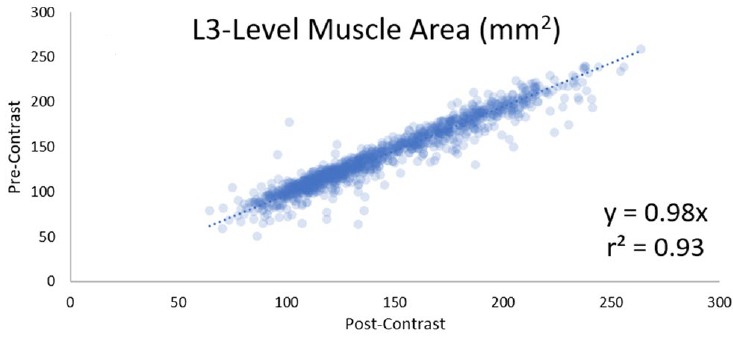
\includegraphics[scale=0.49]{Immagini/perez_areamuscolo.png}\quad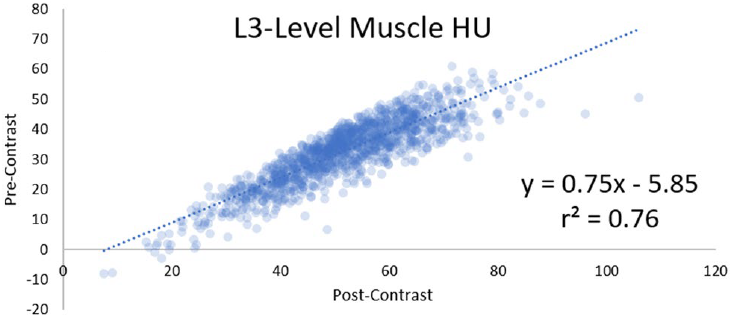
\includegraphics[scale=0.49]{Immagini/perez_attenuazionemuscolo.png}\quad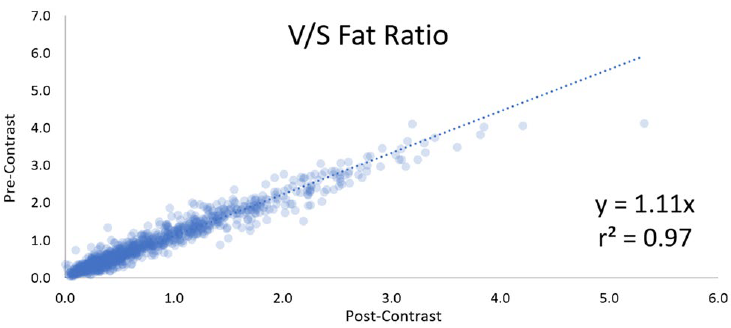
\includegraphics[scale=0.49]{Immagini/perez_vsr.png}\quad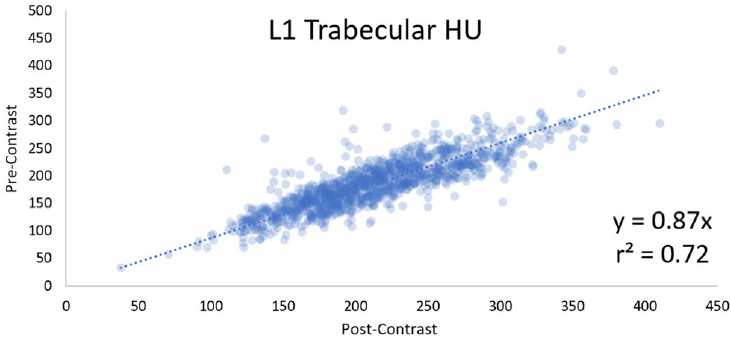
\includegraphics[scale=0.49]{Immagini/perez_trabecole.png}
\caption{\label{fig:perez_correlazioni} \textit{Grafici precontrasto vs postcontrasto di superficie e attenuazione muscolare, misurate a L3, e di VSR e attenuazione trabecolare, misurati a L1. Fonte:} \cite{Perez2021}.}
\end{figure}

L’algoritmo di segmentazione ha commesso alcuni errori con maggiore frequenza di altri nel segmentare le immagini, tra cui parti mancanti durante la segmentazione del muscolo, cattiva segmentazione del grasso in prossimità della fascia muscolare addominale ed erroneo posizionamento della regione d’interesse all'interno della vertebra, con inclusione anche dell'osso corticale (la parte più esterna dell'osso, che va esclusa se si vuole misurare l’attenuazione dell'osso trabecolare); esempi di questi errori sono riportati in \figref{fig:perez_errori}. La soluzione proposta dagli autori è semplicemente quella di utilizzare come \virgolette{ponte} tra TC senza e con contrasto le regressioni lineari trovate, sebbene essi raccomandino anche controlli di validità della segmentazione proposta dall'algoritmo da parte del personale medico preposto.

\begin{figure}[htp]
\centering
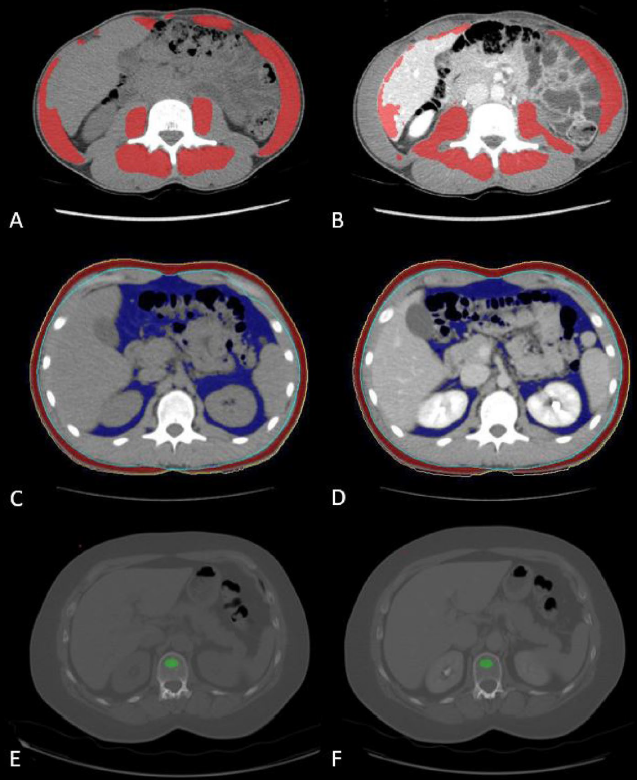
\includegraphics[scale=0.9]{Immagini/perez_errori.png}
\caption{\label{fig:perez_errori} \textit{In alto: segmentazioni precontrasto (A) e postcontrasto (B) di muscolo scheletrico, con evidenti errori di segmentazione in entrambe le immagini. In mezzo: segmentazioni precontrasto (C) e postcontrasto (D) di grasso viscerale (in blu) e sottocutaneo (in rosso); nell'immagine C non si riscontrano errori, mentre nell'immagine D alcune porzioni di grasso viscerale non vengono più riconosciute a causa della differenza nell'attenuazione provocata dall'effetto del mezzo di contrasto. In basso: segmentazioni precontrasto (E) e postcontrasto (F) di osso trabecolare in L1, dove però nell'immagine E la regione di interesse è troppo grande e include anche una parte di osso corticale. Fonte:} \cite{Perez2021}.}
\end{figure}

\section{L'approccio 3D alla segmentazione TC}
Tutti gli studi finora riportati assumono le misure dei tessuti eseguite nella regione T11-L5, e soprattutto per la vertebra L3, come affidabili per la stima della composizione corporea; ciò è dovuto ai numerosi studi che negli ultimi venti anni hanno dimostrato la correlazione fra le misure \textit{single slice} 2D e le misure volumetriche 3D. D’altra parte, sebbene le misure effettuate in 2D rappresentino un buon indicatore per gruppi di studio, ciò non implica che queste stesse misure debbano avere valore prognostico per i singoli pazienti \cite{Ma2021}. In uno studio del 2004 \cite{Shen2004}, Shen \textit{et al.} hanno dimostrato, oltre alla correlazione tra misure 2D e 3D, che considerare diverse \textit{slice} trasversali piuttosto che una sola fornisce una correlazione maggiore. Questa sembra essere l’unica strada percorribile per aumentare l’accuratezza delle misure, dato che l’equazione di regressione trovata in \cite{Shen2004} non può essere generalizzata a tutte le fasce d’età e fra altre categorie di pazienti. Questi dettagli ed altri, che negli studi di gruppo possono essere trascurati per effetto del campione numeroso che si va ad analizzare, possono invece portare ad errori di valutazione per i singoli pazienti, per cui di conseguenza è necessario cercare di condurre analisi il più possibile precise.

Ci sono anche situazioni in cui effettuare misure \textit{single slice} risulta critico, come stimare i volumi e valutare le funzionalità degli organi interni. Per questo motivo, in \cite{Ma2021} viene sottolineata la necessità di sviluppare modelli per il calcolo della composizione corporea non più mediante l’approccio \textit{single slice} ma attraverso misure 3D, possibilmente riguardanti tutto il corpo. Le segmentazioni utilizzate come \textit{ground truth} per l’algoritmo sono state realizzate con un software di segmentazione semiautomatica da degli anatomisti, che hanno preso in considerazione quattro tessuti: muscolo scheletrico (SM), osso, tessuto adiposo sottocutaneo (SAT) e tessuto adiposo viscerale (VAT). Dal \textit{data set} sono state estratte 21 segmentazioni divise in base alla vertebra di riferimento: 4 dalle vertebre cervicali C4-C7, 12 dalle vertebre toraciche T1-T12 e 5 dalle vertebre lombari L1-L5. La segmentazione automatica è stata eseguita mediante la piattaforma DAFS (\textit{Voronoi Health Analytics} \cite{voronoi}), le cui analisi hanno ottenuto dei coefficienti di Dice di 0,980 per l’osso, 0,974 per l’SM, 0,986 per il SAT e 0,960 per il VAT, come si può vedere nella \figref{fig:ma_dice}. In \figref{fig:ma_3d} è riportato un esempio di segmentazione automatica effettuato sulla piattaforma DAFS di alcune immagini TC, insieme alla ricostruzione tridimensionale delle segmentazioni.
\begin{figure}[htp]
\centering
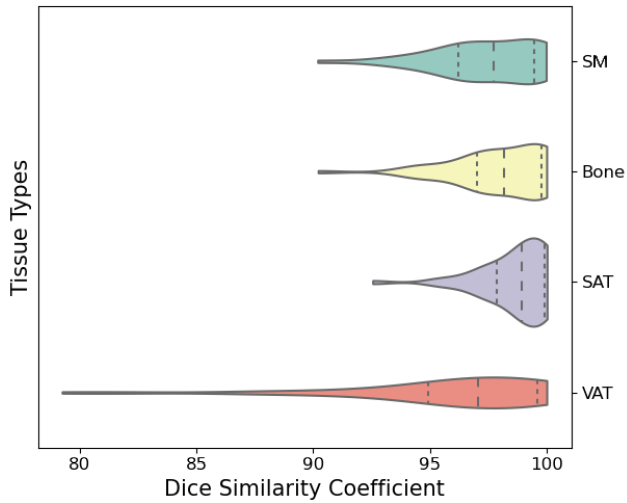
\includegraphics[scale=0.75]{Immagini/ma_dice.png}
\caption{\label{fig:ma_dice} \textit{Diagrammi a violino dei coefficienti di Dice per ogni tessuto. Fonte:} \cite{Ma2021}.}
\end{figure}
\begin{figure}[htp]
\centering
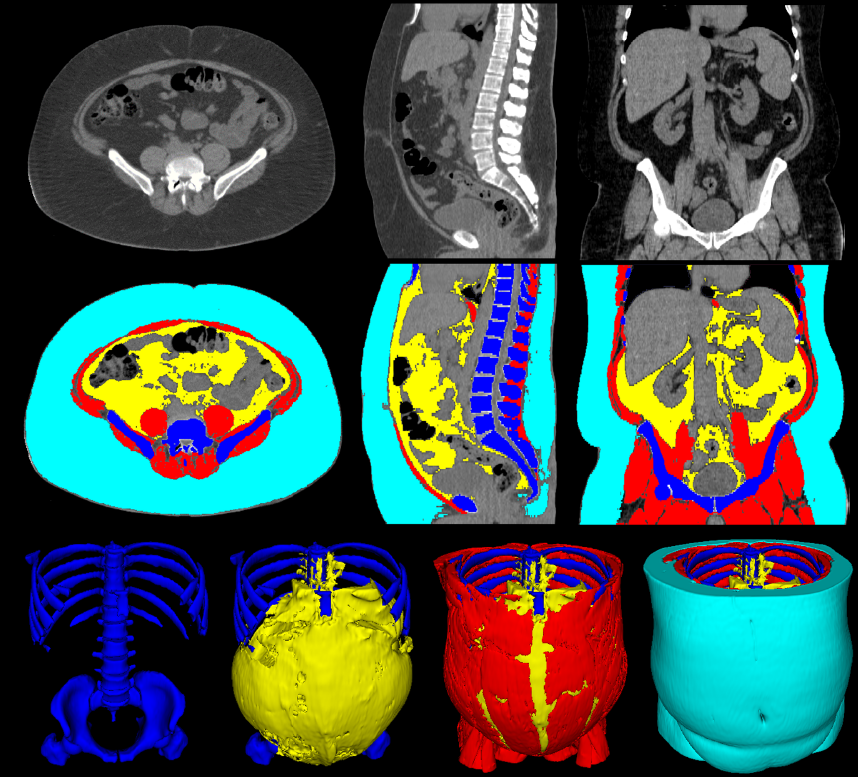
\includegraphics[scale=0.8]{Immagini/ma_3d.png}
\caption{\label{fig:ma_3d} \textit{Da sinistra a destra, visioni assiali, sagittali e coronali di: in alto, immagini TC originali; in mezzo, segmentazioni delle immagini TC di grasso viscerale (giallo), grasso sottocutaneo (azzurro), muscolo (rosso) e osso (blu); in basso, ricostruzione in tre dimensioni dei tessuti segmentati. Fonte:} \cite{Ma2021}.}
\end{figure}

Nella \figref{fig:ma_vertebre} sono rappresentati i risultati di un’analisi \textit{whole body} in termini di volume e attenuazione media di ogni singolo tessuto, indicizzata verticalmente dalle singole vertebre. Si può vedere come l’attenuazione dei diversi tessuti sia piuttosto costante per tutte le vertebre, ma il dato più interessante è rappresentato dalle distribuzioni del SAT e del VAT, che presentano grosse variabilità nei volumi di tessuto nella regione lombare rispetto al resto del corpo. Questi risultati confermano la rappresentatività della vertebra L3 come indicatore valido per stime di composizione corporea, poiché a questa altezza è possibile valutare le differenze in termini di SAT e VAT tra i vari soggetti; in altre parole, la misura delle superfici trasversali dei tessuti nella regione lombare permette la stratificazione dei pazienti sulla base dei volumi di tessuto adiposo. Nonostante ciò, in generale si conferma la problematica, riportata già in \cite{Shen2004}, della non completa validità dell'approccio \textit{single slice} in casi delicati come la definizione dei piani chemioterapici: i modelli di correlazione superficie-volume, infatti, non garantiscono un'accuratezza tale da poter essere utilizzati in ambito clinico, mentre sono accettabili all'interno di studi epidemiologici.

Per concludere, il gruppo di Ma mette in luce in \cite{Ma2021} le potenzialità e il valore dei dati che si potrebbero ottenere da indagini TC 3D, le quali permettono stime molto più accurate della composizione corporea; d’altro canto, se già la segmentazione di una singola \textit{slice} per TC è un processo lungo, se consideriamo che questo processo deve essere ripetuto per più pazienti, la segmentazione di più di una \textit{slice} per paziente, come richiede l’approccio 3D, diventa praticamente impossibile da portare avanti se non con un algoritmo di segmentazione automatica. La piattaforma DAFS, utilizzata dal gruppo di lavoro di Ma, ha ottenuto degli ottimi risultati in termini di coefficiente di similarità di Dice e ha le potenzialità, secondo gli autori del lavoro, di poter implementare col tempo anche \textit{tool} di subsegmentazione, ad esempio misurando il grasso nelle cavità addominali, ventrali e pelviche e suddividendo il grasso di ognuna di queste regioni in regioni anatomiche più piccole. Un software di segmentazione automatica renderebbe anche possibile la misura delle grandezze degli organi interni menzionate prima, sempre perché renderebbe possibile l’applicazione dell'approccio 3D.
\begin{figure}[htp]
\centering
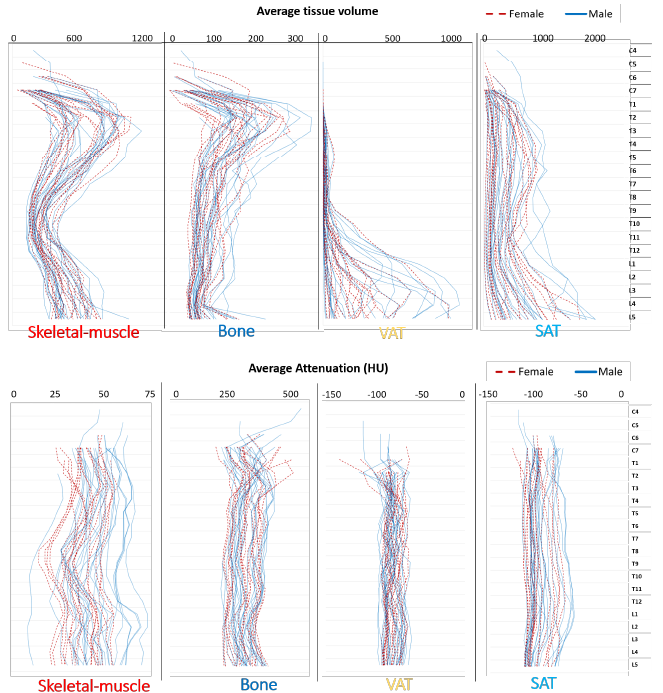
\includegraphics[scale=1.12]{Immagini/ma_vertebre.png}
\caption{\label{fig:ma_vertebre} \textit{Distribuzioni di volumi (in alto) e attenuazioni medie (in basso) per ogni tipo di tessuto e per ogni livello vertebrale. Si può notare un'attenuazione piuttosto costante per tutti i tessuti in entrambi i sessi, mentre i volumi presentano pronunciate variazioni per tutti i tessuti in vertebre diverse, in alcuni casi con differenze importanti anche fra i due sessi. Fonte:} \cite{Ma2021}.}
\end{figure}
\chapter*{Conclusioni}
\addcontentsline{toc}{chapter}{Conclusioni}
L'enorme quantitativo di informazioni contenute all'interno di una TC, una tipologia di esame estremamente versatile e richiesta in gran parte delle specialità mediche per i motivi più disparati, può tornare utile per la stima della composizione corporea dei singoli pazienti. In particolare, misurazioni effettuate mediante TC nella regione lombare sono ritenute altamente rappresentative della composizione corporea del singolo paziente ed è ampiamente dimostrato il loro valore prognostico, soprattutto in caso di tumori. Si potrebbe affermare, in realtà, che i metodi fondati sulla TC non sono solo utili ma quasi necessari, nell'ottica di un progressivo cambiamento degli attuali protocolli per la valutazione della densità minerale ossea, della quantità di grasso, della carenza muscolare e in generale di tutti i metodi mirati, per un motivo o per un altro, alla stima della \textit{body composition}.

È doveroso aggiungere, però, un'importante precisazione: accanto a situazioni in cui i protocolli odierni possono condurre a valutazioni errate dello stato delle cose, e in cui sarebbe invece fondamentale per la salute e la vita del paziente avere informazioni il più precise possibile (è il caso dell'indice di massa corporea usato come estimatore della \textit{body composition} in fase di pianificazione della terapia oncologica), ci sono altre situazioni in cui i metodi odierni non offrono risultati tanto peggiori rispetto alla TC: è il caso, per fare un esempio, della DXA per la valutazione della densità minerale ossea e la diagnosi dell'osteoporosi. In altri casi ancora è stata riscontrata la non adeguatezza degli standard attuali ma neanche della TC, come nel caso di alcuni pazienti colpiti da cancro al polmone, per i quali le grandezze \textit{CT-derived} non sono risultate correlate con la sopravvivenza dei pazienti stessi. In sintesi, la TC è un esame che va valutato con attenzione ma che acquista un enorme valore all'interno dell'approccio di \textit{screening} opportunistico, che prevede l'estrazione di tutti i dati che possono tornare utili da TC che vengono acquisite per altre motivazioni cliniche.

Tuttavia, questi dati possono essere sfruttati a pieno solo mediante metodi di segmentazione automatici, i quali permettono di calcolare quantità come densità, superfici e indici dei diversi tessuti corporei che altrimenti sarebbero impossibili da stimare. I software attualmente disponibili, in particolare le reti neurali a convoluzione, riescono a produrre segmentazioni di immagini TC che dimostrano un ottimo accordo con le segmentazioni effettuate manualmente da radiologi e anatomisti. Un problema da tenere in considerazione durante la progettazione e l'allenamento di un software di questo tipo è l'effetto del mezzo di contrasto sulle grandezze \textit{CT-derived}, che pare essere importante, sebbene al momento non siano presenti studi a sufficienza per avere un'idea consolidata dell'entità del problema.

Infine, un altro importante aspetto della segmentazione dei tessuti in immagini TC per la stima della composizione corporea è l'approccio 3D in contrapposizione al metodo \textit{single slice}: una valutazione della \textit{body composition} sui volumi piuttosto che sulle superfici, infatti, riesce a ottenere risultati molto più accurati, perché permette di superare il problema della rappresentatività delle singole \textit{CT slice}, che per quanto alta (in base al tessuto che consideriamo) non potrà mai essere rappresentativa al 100\% della composizione tissutale di tutto il corpo. L'approccio 3D non potrebbe ovviamente essere praticabile senza la segmentazione automatica, rappresentando un motivo in più per lo sviluppo di software che implementino questa modalità di segmentazione.

\printbibliography[heading=bibintoc]

\chapter*{Ringraziamenti}
A conclusione di questo elaborato, vorrei ringraziare tutte le persone che hanno rivestito una certa importanza nella mia vita durante questi tre anni di percorso universitario.

La Professoressa Claudia Testa, relatrice di questa tesi, per le conoscenze che mi ha fornito nell'ambito della fisica biomedica, e il Dottor David Bianchini, correlatore, per l'estrema disponibilità e competenza dimostrate.

I miei genitori, per avermi sempre lasciato libertà di scelta in ogni ambito della vita e aver sempre supportato ogni mia decisione.

Mia sorella Sara, per esserci sempre nei momenti di bisogno.

I miei nonni, per l'affetto e le premure costanti che mi dimostrano.

Brian, che più di tutti negli ultimi anni mi è stato vicino, che mi ha fatto divertire, crescere, sognare e scoprire come persona e che avrà per sempre un posto nel mio cuore; un grazie speciale.

Francesco, Lidia e Marco, che non perdono mai occasione di dimostrarsi amici sinceri ed affettuosi, anche più di quanto meriti.

Gabriele, che riesce a sopportarmi e a strapparmi un sorriso anche nelle giornate peggiori, nonostante la sua pedanteria e la fissazione con la storia greca.

Tutti i miei compagni di corso, che mi hanno regalato le migliori risate durante le lezioni e fuori, e senza i quali tutto questo sarebbe stato infinitamente più noioso.

A tutti voi, e a molti altri familiari e amici, porgo la più sentita riconoscenza.

\end{document}
